% ---------------------------------------------------------------------------------------------------------------
% TEMPLATE PARA TRABALHO DE CONCLUSÃO DE CURSO
% Universidade Tecnológica Federal do Paraná - UTFPR
% Customização da classe abnTeX2 (http://www.abntex.net.br/) para as normas da UTFPR
%
% Autores: Diego Marczal
% 	       Michael Vornes <https://github.com/mvornes>
% Adaptação (DACOM-CP): Silvio Ricardo Rodrigues Sanches
%
%----------------------------------------------------------------------------------------------------------------
% Codificação: UTF-8
% LaTeX:  abnTeX2          
% ---------------------------------------------------------------------------------------------------------------


% CARREGA CLASSE PERSONALIZADA DA UTFPR--------------------------------------------------------------------------
\documentclass[%twoside,                   % Impressão em frente e verso
    	        oneside,                   % Impressão apenas frente
]{configuracoes/utfpr-abntex2}


% INCLUI ARQUIVOS DE CONFIGURAÇÕES-------------------------------------------------------------------------------
% REFERÊNCIAS------------------------------------------------------------------
\usepackage[%
    alf,
    abnt-emphasize=bf,
    bibjustif,
    recuo=0cm,
    abnt-url-package=url,       % Utiliza o pacote url
    abnt-refinfo=yes,           % Utiliza o estilo bibliográfico abnt-refinfo
    abnt-etal-cite=3,
    abnt-etal-list=3,
    abnt-thesis-year=final
]{abntex2cite}                  % Configura as citações bibliográficas conforme a norma ABNT

% PACOTES----------------------------------------------------------------------
\usepackage[utf8]{inputenc}                                 % Codificação do documento
\usepackage[T1]{fontenc}                                    % Seleção de código de fonte
\usepackage{booktabs}                                       % Réguas horizontais em tabelas
\usepackage{color, colortbl}                                % Controle das cores
\usepackage{float}                                          % Necessário para tabelas/figuras em ambiente multi-colunas
\usepackage{graphicx}                                       % Inclusão de gráficos e figuras
\usepackage{icomma}                                         % Uso de vírgulas em expressões matemáticas
\usepackage{indentfirst}                                    % Indenta o primeiro parágrafo de cada seção
\usepackage{microtype}                                      % Melhora a justificação do documento
\usepackage{multirow, array}                                % Permite tabelas com múltiplas linhas e colunas
\usepackage{subeqnarray}                                    % Permite subnumeração de equações
\usepackage{lastpage}                                       % Para encontrar última página do documento
\usepackage{verbatim}                                       % Permite apresentar texto tal como escrito no documento, ainda que sejam comandos Latex
\usepackage{amsfonts, amssymb, amsmath}                     % Fontes e símbolos matemáticos
\usepackage[algoruled, portuguese]{algorithm2e}             % Permite escrever algoritmos em português
%\usepackage[scaled]{helvet}                                % Usa a fonte Helvetica
\usepackage{times}                                          % Usa a fonte Times
%\usepackage{palatino}                                      % Usa a fonte Palatino
%\usepackage{lmodern}                                       % Usa a fonte Latin Modern
\usepackage[bottom]{footmisc}                               % Mantém as notas de rodapé sempre na mesma posição
\usepackage{ae, aecompl}                                    % Fontes de alta qualidade
\usepackage{latexsym}                                       % Símbolos matemáticos
\usepackage{lscape}                                         % Permite páginas em modo "paisagem"
%\usepackage{picinpar}                                      % Dispor imagens em parágrafos
%\usepackage{scalefnt}                                      % Permite redimensionar tamanho da fonte
%\usepackage{subfig}                                        % Posicionamento de figuras
%\usepackage{upgreek}                                       % Fonte letras gregas

% For subfigures
%\usepackage[demo]{graphicx}
\usepackage{caption}
\usepackage{subcaption}

% For code snippet
\usepackage{listings}
\usepackage{color}

% Redefine a fonte para uma fonte similar a Arial (fonte Helvetica)
\renewcommand*\familydefault{\sfdefault}

% CONFIGURAÇÕES DE APARÊNCIA DO PDF FINAL--------------------------------------
\makeatletter
\hypersetup{%
    portuguese,
    colorlinks=true,   % true: "links" coloridos; false: "links" em caixas de texto
    linkcolor=blue,    % Define cor dos "links" internos
    citecolor=blue,    % Define cor dos "links" para as referências bibliográficas
    filecolor=blue,    % Define cor dos "links" para arquivos
    urlcolor=blue,     % Define a cor dos "hiperlinks"
    breaklinks=true,
    pdftitle={\@title},
    pdfauthor={\@author},
    pdfkeywords={abnt, latex, abntex, abntex2}
}
\makeatother

% ALTERA O ASPECTO DA COR AZUL--------------------------------------------------
\definecolor{blue}{RGB}{41,5,195}

% REDEFINIÇÃO DE LABELS---------------------------------------------------------
\renewcommand{\algorithmautorefname}{Algoritmo}
\def\equationautorefname~#1\null{Equa\c c\~ao~(#1)\null}

% CRIA ÍNDICE REMISSIVO---------------------------------------------------------
\makeindex

% HIFENIZAÇÃO DE PALAVRAS QUE NÃO ESTÃO NO DICIONÁRIO---------------------------
\hyphenation{%
    qua-dros-cha-ve
    Kat-sa-gge-los
}

\definecolor{dkgreen}{rgb}{0,0.6,0}
\definecolor{gray}{rgb}{0.5,0.5,0.5}
\definecolor{mauve}{rgb}{0.58,0,0.82}

\lstset{frame=tb,
  language=Python,
  aboveskip=3mm,
  belowskip=3mm,
  showstringspaces=false,
  columns=flexible,
  basicstyle={\small\ttfamily},
  numbers=none,
  numberstyle=\tiny\color{gray},
  keywordstyle=\color{blue},
  commentstyle=\color{dkgreen},
  stringstyle=\color{mauve},
  breaklines=true,
  breakatwhitespace=true,
  tabsize=3
}

\renewcommand{\lstlistingname}{Listagem}


% INCLUI ARQUIVOS DO TRABALHO DE CONCLUSÃO DE CURSO (PRÉ-TEXTUAIS, TEXTUAIS, PÓS-TEXTUAIS)-----------------------

% INSERE CAPA E FOLHA DE ROSTO
% CAPA---------------------------------------------------------------------------------------------------

% ORIENTAÇÕES GERAIS-------------------------------------------------------------------------------------
% Caso algum dos campos não se aplique ao seu trabalho, como por exemplo,
% se não houve coorientador, apenas deixe vazio.
% Exemplos: 
% \coorientador{}
% \departamento{}

% DADOS DO TRABALHO--------------------------------------------------------------------------------------
\titulo{Análise de dados acadêmicos para construção de mecanismos de apoio a redução da retenção no ensino superior}

% \titulo{Aplicação de técnicas de ciência de dados para análise de dados acadêmicos e construção de mecanismos de apoio a redução da retenção no ensino superior.}

\titleabstract{Title in English}
\autor{Lucas Ricardo de Lima Franco}
\autorcitacao{FRANCO, Lucas R. L.} % Sobrenome em maiúsculo
\local{Cornélio Procópio}
\data{2019}

% NATUREZA DO TRABALHO-----------------------------------------------------------------------------------
% Opções: 
% - Trabalho de Conclusão de Curso (se for Graduação)
% - Dissertação (se for Mestrado)
% - Tese (se for Doutorado)
% - Projeto de Qualificação (se for Mestrado ou Doutorado)
\projeto{Trabalho de Conclusão de Curso}

% TÍTULO ACADÊMICO---------------------------------------------------------------------------------------
% Opções:
% - Bacharel ou Tecnólogo (Se a natureza for Trabalho de Conclusão de Curso)
% - Mestre (Se a natureza for Dissertação)
% - Doutor (Se a natureza for Tese)
% - Mestre ou Doutor (Se a natureza for Projeto de Qualificação)
\tituloAcademico{Bacharel}

% ÁREA DE CONCENTRAÇÃO E LINHA DE PESQUISA---------------------------------------------------------------
% Se a natureza for Trabalho de Conclusão de Curso, deixe ambos os campos vazios
% Se for programa de Pós-graduação, indique a área de concentração e a linha de pesquisa
\areaconcentracao{}
\linhapesquisa{}

% DADOS DA INSTITUIÇÃO-----------------------------------------------------------------------------------
% Se a natureza for Trabalho de Conclusão de Curso, coloque o nome do curso de graduação em "programa"
% Formato para o logo da Instituição: \logoinstituicao{<escala>}{<caminho/nome do arquivo>}
\instituicao{Universidade Tecnológica Federal do Paraná}
\departamento{Departamento Acadêmico de Computação}
\programa{Engenharia de Computação}
\logoinstituicao{0.2}{dados/figuras/logo-instituicao.png} 

% DADOS DOS ORIENTADORES---------------------------------------------------------------------------------
\orientador{Francisco Pereira Junior}
%\orientador[Orientadora:]{Nome da orientadora}
\instOrientador{Universidade Tecnológica Federal do Paraná}

\coorientador{}
%\coorientador[Coorientadora:]{Nome da coorientadora}
\instCoorientador{}

% FOLHA DE ROSTO--------------------------------------------------------------------------------------------------------

% TRABALHO DE CONCLUSÃO DE CURSO
 \preambulo{{\imprimirprojeto} apresentado ao curso de {\imprimirprograma} da {\imprimirinstituicao}, como requisito parcial para a obtenção do título de {\imprimirtituloAcademico}.}

% DISSERTAÇÃO DE MESTRADO
% \preambulo{{\imprimirprojeto} apresentada ao Programa de \mbox{Pós-graduação} da {\imprimirinstituicao}, como requisito parcial para obtenção do título de {\imprimirtituloAcademico}.}

% TESE DE DOUTORADO
% \preambulo{{\imprimirprojeto} apresentada ao Programa de \mbox{Pós-graduação} da {\imprimirinstituicao}, como requisito parcial para a obtenção do título de {\imprimirtituloAcademico}.}

% PROJETO DE QUALIFICAÇÃO DE MESTRADO OU DOUTORADO
%\preambulo{{\imprimirprojeto} apresentado ao Programa de \mbox{Pós-graduação} da {\imprimirinstituicao}, como requisito parcial para a obtenção do título de {\imprimirtituloAcademico}.}

% OBSERVAÇÕES-----------------------------------------------------------------------------------------------------------
% Altere este arquivo APENAS comentando as linhas que não se aplicam ao tipo de trabalho acadêmico desejado.


\begin{document}

\pretextual
\imprimircapa                                               	           % Comando para imprimir Capa
\imprimirfolhaderosto{}                                     		   % Comando para imprimir Folha de rosto
% INSERE ELEMENTOS PRÉ-TEXTUAIS
% % DEDICATÓRIA------------------------------------------------------------------

\renewcommand{\dedicatorianame}{DEDICATÓRIA}

\begin{dedicatoria}

Altere este texto inserindo a dedicatória do seu trabalho. 

\end{dedicatoria}
          			   % Dedicatória
% AGRADECIMENTOS---------------------------------------------------------------

\begin{agradecimentos}[AGRADECIMENTOS]

Primeiramente agradeço a Deus por ter me dado a oportunidade e vigor para chegar até aqui.

Agradeço ao professor orientador Francisco Pereira Junior (Thesko), por todo o apoio e empenho dedicado para a realização deste trabalho e a todos os professores por todas as contribuições dadas, que reunidas fortaleceram muito mais do que o profissional, mas o humano que sou.

Agradeço também à toda a minha famı́lia, principalmente meus pais, meus irmãos e avôs, por todo o incentivo, hoje percebo que sem eles nada disso seria possível. 

E deixo aqui registrado a importância dos meus amigos em todos os momentos dessa jornada, pois percebo também o quanto cresci e aprendi com eles, e quanto o coletivo foi importante para a construção do indivíduo de cada um de nós.

Por fim agradeço a todos que direta ou indiretamente fizeram parte desta jornada.

\end{agradecimentos}
        			   % Agradecimentos
% EPÍGRAFE---------------------------------------------------------------------

\renewcommand{\epigraphname}{EPÍGRAFE}

\begin{epigrafe}

\textit{“Não vemos as coisas como elas são, mas como nós somos.” (Anaïs Nin)}

\end{epigrafe}

% OBSERVAÇÕES------------------------------------------------------------------
% Altere o texto para inserir a epígrafe do seu trabalho
              			   % Epígrafe
% RESUMO--------------------------------------------------------------------------------

\begin{resumo}[RESUMO]
\begin{SingleSpacing}

% Não altere esta seção do texto--------------------------------------------------------
\imprimirautorcitacao. \imprimirtitulo. \imprimirdata. \pageref {LastPage} f. \imprimirprojeto\ – \imprimirprograma, \imprimirinstituicao. \imprimirlocal, \imprimirdata.\\
%---------------------------------------------------------------------------------------

A retenção no ensino superior é um fenômeno complexo que causa grandes impactos na sociedade, devido a todos os fatores que estão intrinsecamente relacionados com sua ocorrência, como o financeiro, educacional e social.
Este trabalho tem a retenção como objeto de estudo e apresenta a construção de um sistema para análise de dados acadêmicos utilizando técnicas de mineração de dados.
Em conjunto são implementados mecanismos automáticos para comunicação com alunos e artifícios para que docentes possam extrair \textit{insights} e tomar ações a fim de contribuir para a redução da retenção acadêmica.
\\

\textbf{Palavras-chave}:
Aprendizado de máquina. Ensino superior. Reconhecimento de padrões. Retenção acadêmica. Sistema acadêmico.

\end{SingleSpacing}
\end{resumo}

% OBSERVAÇÕES---------------------------------------------------------------------------
% Altere o texto inserindo o Resumo do seu trabalho.
% Escolha de 3 a 5 palavras ou termos que descrevam bem o seu trabalho 
             			   % Resumo em Português
% ABSTRACT--------------------------------------------------------------------------------

\begin{resumo}[ABSTRACT]
\begin{SingleSpacing}

% Não altere esta seção do texto--------------------------------------------------------
\imprimirautorcitacao. \imprimirtitleabstract. \imprimirdata. \pageref {LastPage} f. \imprimirprojeto\ – \imprimirprograma, \imprimirinstituicao. \imprimirlocal, \imprimirdata.\\
%---------------------------------------------------------------------------------------

\textbf{Keywords}: 

\end{SingleSpacing}
\end{resumo}

% OBSERVAÇÕES---------------------------------------------------------------------------
% Altere o texto inserindo o Abstract do seu trabalho.
% Escolha de 3 a 5 palavras ou termos que descrevam bem o seu trabalho 
             		           % Resumo em Inglês
% LISTA DE ABREVIATURAS E SIGLAS----------------------------------------------------------

\begin{siglas}
    \item[ACID] Atomicidade, Consistência, Isolamento e Durabilidade
    \item[AVA] Ambiente Virtual de Aprendizagem
    \item[BD] Banco de Dados
    \item[CSS] \textit{Cascading Style Sheets}
    \item[CRISP-DM] \textit{Cross-Industry Standard Process for Data Mining}
    \item[CRUB] Conselho de Reitores das Universidades Brasileiras
    \item[CSV] \textit{Comma Separated Values}
    \item[HTML] \textit{Hypertext Markup Language}
    \item[IES] Instituições de Ensino Superior
    \item[IFES] Instituições Federais de Ensino Superior
    \item[INEP] Instituto Nacional de Estudos e Pesquisas Educacionais Anísio Teixeira
    \item[IoT] \textit{Internet of Things}
    \item[KDD] \textit{Knowledge Discovery in Databases}
    \item[JSON] \textit{JavaScript Object Notation}
    \item[Moodle] \textit{Modular Object-Oriented Dynamic Learning Environment}
    \item[MD]   Mineração de Dados
    \item[ML]   \textit{Machine Learning}
    \item[R.A.] Registro Acadêmico
    \item[SPA] \textit{Single Page Application}
    \item[UFRGS] Universidade Federal do Rio Grande do Sul
    \item[URL] \textit{Uniform Resource Locator}
    \item[UTFPR] Universidade Tecnológica Federal do Paraná
    \item[USP] Universidade de São Paulo
    \item[WEKA] \textit{Waikato Environment for Knowledge Analysis}
    \item[XML] \textit{eXtensible Markup Language}
\end{siglas}

% OBSERVAÇÕES-----------------------------------------------------------------------------
% Altere a lista acima para definir os acrônimos e siglas utilizados neste trabalho
          		   % Lista de Abreviaturas e Siglas
% Lista de Figuras----------------------------------------------------------------

\pdfbookmark[0]{\listfigurename}{lof}
\listoffigures*
\cleardoublepage

% OBSERVAÇÕES---------------------------------------------------------------------
% Este arquivo não precisa de ser alterado, pois a lista é gerada automaticamente.
   % Lista de Figuras
% % LISTA DE QUADROS----------------------------------------------------------------

\renewcommand{\listofquadrosname}{LISTA DE QUADROS}

\pdfbookmark[0]{\listofquadrosname}{loq}
\listofquadros*
\cleardoublepage

% OBSERVAÇÕES---------------------------------------------------------------------
% Este arquivo não necessita de ser editado. A lista é gerada automaticamente.
   % Lista de Quadros
% LISTA DE TABELAS-------------------------------------------------------------

\pdfbookmark[0]{\listtablename}{lot}
\listoftables*
\cleardoublepage

% OBSERVAÇÕES-------------------------------------------------------------------
% Este arquivo não precisa ser alterado, pois a lista é gerada automaticamente.
         		   % Lista de Tabelas
% % LISTA DE SÍMBOLOS------------------------------------------------------------

\begin{simbolos}
    \item[$ \Gamma $] Letra grega Gama
    \item[$ \lambda $] Comprimento de onda
    \item[$ \in $] Pertence
\end{simbolos}

% OBSERVAÇÕES-------------------------------------------------------------------
% Altere a lista acima para definir os símbolos utilizados no trabalho
        		   % Lista de Símbolos
% % LISTA DE ALGORITMOS----------------------------------------------------------

\newcommand{\algoritmoname}{Algoritmo}
\renewcommand{\listalgorithmcfname}{LISTA DE ALGORITMOS}

\floatname{algocf}{\algoritmoname}
\newlistof{listofalgoritmos}{loa}{\listalgoritmoname}
\newlistentry{algocf}{loa}{0}

\counterwithout{algocf}{chapter}
\renewcommand{\cftalgocfname}{\algoritmoname\space}
\renewcommand*{\cftalgocfaftersnum}{\hfill--\hfill}

\pdfbookmark[0]{\listalgorithmcfname}{loa}
\listofalgorithms
\cleardoublepage

% OBSERVAÇÕES------------------------------------------------------------------
% Este arquivo não precisa ser alterado, pois a lista é gerada automaticamente.
   % Lista de Algoritmos
% SUMÁRIO----------------------------------------------------------------------

\renewcommand{\contentsname}{SUMÁRIO}

\pdfbookmark[0]{\contentsname}{toc}
\tableofcontents*
\cleardoublepage

% OBSERVAÇÕES-------------------------------------------------------------------
% Este arquivo não precisa ser alterado, pois o sumário é gerado automaticamente.
               			   % Sumário

\textual
% INSERE ELEMENTOS TEXTUAIS
\chapter{INTRODUÇÃO}
\label{chap:introducao}

A evasão e a retenção acadêmica no ensino superior são fenômenos que possuem várias vertentes e trazem muitas discussões. Isto porque envolve fatores que não estão somente relacionados ao ensino e a educação, mas à outros tópicos importantes para a sociedade, como o viés econômico. Segundo \citeonline{SilvaFilho2007}, fundadores do Instituto Lobo, que tem como objetivo contribuir com soluções para os problemas brasileiros relacionados às áreas de educação, ciência e tecnologia, o desperdício de recursos devido a evasão tanto em Instituições de Ensino Superior (IES) públicas quanto privadas é de mais de dez bilhões de reais anualmente, e mesmo que seja um tema discutido, não recebe a devida importância e ações necessárias.

\citeonline{SilvaFilho2007} apresentam também, baseado em estudos nacionais e internacionais feitos pelo Instituto Lobo, uma lista de ações consideradas bem-sucedidas para o combate e redução da evasão nas IES brasileiras. A seguir são apresentadas algumas destas ações.

\begin{enumerate}
    \item Análise estatística do fenômeno da evasão;
    \item Criação de programas de aconselhamento e orientação de alunos;
    \item Envolvimento da comunidade acadêmica no combate à evasão estimulando a visão centrada no aluno;
    \item Criação de condições que satisfaçam os objetivos responsáveis por atrair os alunos às IES e apresentar casos positivos de satisfação;
    \item Modernização da forma como são ministrados os cursos:
    \item Introdução de atividades relacionadas à profissões desde o início do curso;
    \item Estímulo para o desenvolvimento de atitudes inovadoras e empreendedoras pelos estudantes.
\end{enumerate} 

Além das ações consideradas convencionais apresentadas, existem também ações tecnológicas, que podem ser aplicadas a fim de torná-las mais eficientes, como por exemplo a implementação de Sistemas Inteligentes. 
Desenvolvidos respeitando as especificidades de cada instituição, estes sistemas podem auxiliar no acompanhamento do desempenho de alunos, professores e cursos, possibilitando a identificação de situações "críticas", como a de alunos que apresentam grande possibilidade de reprovação ou evasão, dificuldades pedagógicas por conta de professores, disciplinas com altos índices de reprovação e os possíveis motivos para estas ocorrências.

Das ações apresentadas, a número 1 é a que mais se enquadra ao escopo deste trabalho, que visou, a partir da análise de dados acadêmicos, compreender a retenção no ensino superior, descrever estratégias que possibilitem predizer a situação de alunos e dar suporte para que outros grupos (pedagogos, assistentes estudantis e professores) usufruam e tomem ações a partir delas. 

\section{PROBLEMA}
\label{sec:problema}

Evidencia-se em números a problemática que se inserem as IES brasileiras quando trata-se da \textbf{evasão} e da \textbf{retenção}. Temas delicados devido a natureza subjetiva dos motivos que levam ao acontecimento, os índices de desistência e reprovação no Ensino Superior cresceu consideravelmente nos últimos anos, apresentando um aumento de mais de 37\% entre os anos de 2010 e 2014, segundo o Censo da Educação Superior 2015, divulgado pelo \citeonline{INEP2016}. 

Segundo \citeonline{Santos2018}, o número de vagas ociosas nas instituições federais brasileiras é de mais de 25\% do total de vagas ofertadas, devido à evasão e ao não preenchimento destas em processos seletivos. Nas instituições estaduais estes números aproximam-se de 17\%.

\citeonline{SilvaFilho2007} argumentam em seu trabalho que essa ociosidade de vagas na educação superior gera, além da perda da qualificação profissional dos estudantes, impactos econômicos negativos para a nação como um todo, uma vez que, os recursos públicos que foram aplicados para a criação destas vagas não surtiram um retorno correspondente.

E, como destacado por \citeonline{Marques2015}, o contexto de dados acadêmicos pode envolver um considerável volume de dados, uma vez que este pode ser escalável e evoluir para diferentes instituições de ensino.
Além do volume, tem-se a substancial variedade dos dados, já que cada docente possui certa autonomia para estruturar as disciplinas vinculadas da forma que lhe convém, considerando ainda diferentes instituições de ensino, com diferentes padrões de avaliação.

\section{JUSTIFICATIVA}
\label{sec:justificativa}
Devido a atual situação das IES em relação as taxas de retenção, se faz necessário a criação de ferramentas que tornem possível agir sobre a retenção em cursos de graduação, reduzindo estes números. Além de traçar perfis que permitam compreender o comportamento dos alunos e predizer possíveis situações a partir da análise de dados acadêmicos prévios. 

\section{OBJETIVOS}
\label{sec:objetivos}

O objetivo geral deste trabalho é a análise de dados acadêmicos e o desenvolvimento de uma plataforma utilizando técnicas de mineração de dados, a fim de permitir uma análise mais profunda dos dados acadêmicos por conta dos usuários, permitindo assim extrair \textit{insights} e construir mecanismos de apoio à redução da retenção no ensino superior.

\subsection{Objetivos Específicos}

\begin{itemize}
    \item Construção de gráficos para fácil apresentação e análise de dados;
    \item Implementação de algoritmos de aprendizado de máquina e reconhecimento de padrões que atuem a fim de identificar e prever a retenção em cursos de graduação; 
    \item Desenvolvimento de um sistema web para que docentes tenham acesso aos dados acadêmicos, gráficos e mecanismos;    
    \item Desenvolvimento de mecanismos automatizados que possibilitem a comunicação com alunos em determinadas situações, como a situação de risco de reprovação por faltas em determinada disciplina.
\end{itemize}

\section{ORGANIZAÇÃO DO TRABALHO}
\label{sec:organizacaoTrabalho}

Este trabalho é dividido em cinco capítulos. 
O capítulo dois contém a fundamentação teórica, apresentando a contextualização de temas pertinentes ao trabalho e a revisão da literatura realizada. 
O capítulo três descreve a proposta de trabalho, destacando as tecnologias e ferramentas utilizadas, as etapas executadas com o processo metodológico utilizado e o detalhamento da implementação efetuada apresentando cada uma das partes do sistema desenvolvido.
O capítulo seguinte apresenta a análise dos resultados, levando em conta os modelos de predição e o sistema implementado. 
E o último capítulo contém as considerações finais apresentadas para este trabalho.                		     % REVISÃO DE LITERATURA--------------------------------------------------------

\chapter{FUNDAMENTAÇÃO TEÓRICA}
\label{chap:fundamentacaoTeorica}

Nesta seção são apresentados os conceitos básicos abordados neste trabalho. 
Inicialmente serão contextualizadas a evasão e a retenção acadêmica.
Nas seções seguintes são abordados os conceitos de mineração de dados; o CRISP-DM, modelo de processo utilizado em projetos de mineração de dados; e, de visualização de dados.

\section{EVASÃO E RETENÇÃO NO ENSINO SUPERIOR}

A retenção no ensino superior é o objeto principal da aplicação deste trabalho, porém devido a relação intrínseca que esta possui com a evasão acadêmica, ambos serão melhor contextualizados.

A evasão e a retenção acadêmica são temas muito discutidos devido a importância e aos impactos sociais e econômicos que trazem consigo.

Em 1995 ocorreu o Seminário sobre evasão nas Universidades Brasileiras, evento promovido pelo Conselho de Reitores das Universidades Brasileiras (CRUB), que divulgou indicadores que apontavam uma taxa de evasão média consideravelmente elevada para as Instituições Federais de Ensino Superior (IFES).
A partir do evento constituiu-se uma comissão especial para estudos sobre a evasão nas IES públicas \cite{Pereira2003, SESu1997, Silva2012}.

Esta comissão definiu os conceitos básicos que caracterizam à evasão, distinguindo-as da seguinte forma:

\begin{itemize}
    \item \textbf{Evasão de curso:} ocorre quando o aluno desliga-se do curso superior, podendo caracterizar-se por abandono (deixar de efetuar a matrícula), desistência, transferência ou reopção de curso, trancamento ou exclusão por norma institucional.
    \item \textbf{Evasão da instituição:} ocorre quando o estudante desliga-se da instituição na qual está matriculado.
    \item \textbf{Evasão do sistema:} ocorre quando o estudante abandona temporariamente ou definitivamente o ensino superior.
\end{itemize}

E em relação aos fatores que podem levar um aluno a evasão acadêmica, estes são descritos como:

\begin{itemize}
    \item \textbf{Fatores individuais do aluno:} relacionados à personalidade, ao interesse pelo curso e a expectativa do aluno quanto ao curso escolhido.
    \item \textbf{Fatores internos à instituição:} relacionados à questões acadêmicas, como a falta de formação pedagógica dos docentes, infraestrutura de pouca qualidade ou ausência de um sistema de apoio psicopedagógico ao aluno.
    \item \textbf{Fatores externos à instituição:} são fatores dos quais a instituição tem pouca predominância, como às condições familiar, social e financeira do estudante e o mercado de trabalho.
\end{itemize}

Já a retenção acadêmica é definida como a não seriação apropriada de um aluno devido à reprovação, ou seja, um atraso que faz com que seja necessário cursar disciplinas de períodos letivos anteriores ao esperado que o aluno esteja cursando. Pode-se distinguir a retenção em razão das suas características como:

\begin{itemize}
    \item \textbf{Retenção parcial:} ocorre quando o aluno se encontra em atraso antes do tempo estipulado para término do curso, podendo ainda reverter a situação;
    \item \textbf{Retenção total:} ocorre quando o aluno extrapola o tempo estipulado para término do curso.
\end{itemize}

\citeonline{Lamers2017} apresentam em seu trabalho um estudo de caso sobre a evasão e retenção no curso de Odontologia da Universidade Federal do Rio Grande do Sul (UFRGS). 
Neste os autores efetuam pesquisas com discentes e docentes a fim de identificar os fatores de maior influência para a ocorrência de retenção ou evasão, estas são exibidas na \autoref{fig:evasao-retencao}.

\begin{figure}[!htb]
    \centering
    \caption{Fatores de destaque em relação à retenção e à evasão, segundo estudantes e professores do curso de Odontologia da UFRGS}
    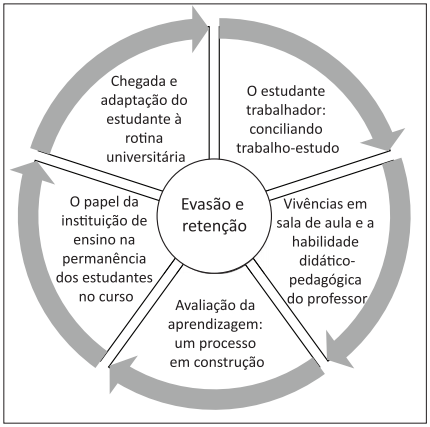
\includegraphics[width=0.6\textwidth]{./dados/figuras/proposta/evasao-retencao}
    \fonte{\citeonline{Lamers2017}}
    \label{fig:evasao-retencao}
\end{figure}

Assim, a possibilidade de antever o desempenho dos estudantes em disciplinas do ensino superior dentro de um espaço de tempo pode ser muito relevante, uma vez que pode-se tomar ações acerca dessa situação e se possível revertê-la.

Neste contexto, a mineração de dados pode ser empregada, com o uso de técnicas de aprendizado de máquina, a fim de realizar a detecção de padrões e definição de modelos que descrevam o comportamento da situação em discussão. Claramente, devido a natureza subjetiva do ambiente acadêmico, o número de variáveis que influenciam no desempenho dos alunos é muito grande, desta forma a acurácia associada à predição se torna muito dependente da qualidade, confiabilidade e volume dos dados disponíveis \cite{Caetano2016}.

A seguir é contextualizada a mineração de dados, bem como algumas de suas técnicas.

\section{MINERAÇÃO DE DADOS}
\label{sec:mineracaoDados}

Embora inicialmente direcionadas as áreas de negócios, as técnicas de mineração de dados se tornaram grandes ferramentas para a extração de conhecimento a partir de volumes de dados, e atualmente, diversos setores a utilizam para o reconhecimento de padrões e análise de dados \cite{Marques2015}.

\citeonline{Weis1999} definem a mineração de dados como a busca e extração de informações valiosas de grandes volumes de dados, com a cooperação entre o homem - que projeta os bancos de dados, descreve os problemas e define os objetivos desejados, e o computador - que verifica os dados buscando padrões que harmonizem com as metas definidas anteriormente. Muitos autores classificam a mineração de dados como a mistura dos campos de estudo da estatística, da inteligência artificial e dos bancos de dados \cite{Cortes2002}.

Para este trabalho foram empregadas técnicas de mineração de dados e aprendizado de máquina como forma de extração de informação e predição dos volumes de dados acadêmicos. A seguir são apresentadas as técnicas de mineração de dados utilizadas neste trabalho.

\subsection{Ferramentas Estatísticas}
    
A primeira técnica consiste das ferramentas estatísticas, utilizadas para efetuar análises simples do conjunto de dados a ser minerado. Muitas vezes com estas ferramentas é possível extrair informações relevantes sobre a distribuição dos conjuntos de dados. Alguns exemplos destas ferramentas são a média aritmética, valores mínimos e máximos, desvio padrão e a distribuição percentual dos dados.

Com estas informações é possível construir gráficos e outras ferramentas visuais que possibilitam uma análise inicial dos dados \cite{Adriaans1996}.

\subsection{Regressão Linear}
A regressão linear é uma técnica de predição numérica, e tem como objetivo estimar valores futuros para uma variável contínua, tentando encontrar uma relação com comportamento linear entre as variáveis preditoras.
Ou seja, onde é possível criar um modelo no qual o valor de uma variável \textit{y} pode ser descrita como uma função linear de uma variável \textit{x}.
Para esta técnica as variáveis preditoras são os atributos do conjunto de dados e usualmente é utilizada a abordagem dos mínimos quadrados para otimizar a função, minimizando a soma dos quadrados das diferenças entre o valor estimado e os dados reais \cite{Camilo2009}.
    
A \autoref{fig:regressao-linear} apresenta um exemplo de regressão linear, no qual é possível verificar uma relação entre as variáveis envolvidas por meio da linearidade entre elas.
Nesta verifica-se que o comportamento da variável 'Salários Mínimos' pode ser descrito aproximadamente como uma função linear da variável 'Anos de Experiências'. A linha contínua representa um exemplo de função linear que seria retornado por um modelo de regressão linear para este conjunto de dados.
    
\begin{figure}[!htb]
    \centering
    \caption{Exemplo de regressão linear, com a variável 'Salários Mínimos' em função da variável 'Anos de Experiências'}
    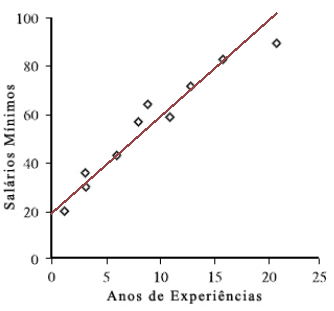
\includegraphics[width=0.5\textwidth]{./dados/figuras/proposta/regressao-linear2}
    \fonte{\citeonline{Camilo2009}}
        \label{fig:regressao-linear}(Adaptado)
    \end{figure}

\subsection{Arvore de Decisão}

A árvore de decisão é um método simples de aprendizado de máquina construído por um processo chamado de indução, que visa dividir os dados em subconjuntos de forma a entender as segmentações criadas para cada atributo, ou \textit{feature}, do modelo. 

Ela funciona como um fluxograma no formato de árvore, onde cada nó não folha apresenta um teste realizado sobre um valor, as ligações entre os nós possuem os valores possíveis para o teste efetuado, e os nós folha indicam a classe ao qual o registro foi determinado como pertencente.

Apesar da simplicidade do método, a árvore de decisão apresenta acurácia semelhante a de métodos mais complexos, porém demanda de uma análise detalhada dos dados para garantir que bons resultados sejam obtidos  \cite{Camilo2009}.

A \autoref{fig:arvore-decisao} apresenta um exemplo simplificado de árvore de decisão, onde é classificado a partir do atributo idade de uma determinada amostra a classe ao qual esta pertence. Os retângulos representam as regras ou testes, e as possíveis classes são representadas pelas elipses.

\begin{figure}[!htb]
    \centering
    \caption{Exemplo simplificado de árvore de decisão, com a classificação de faixa etária por meio da idade}
    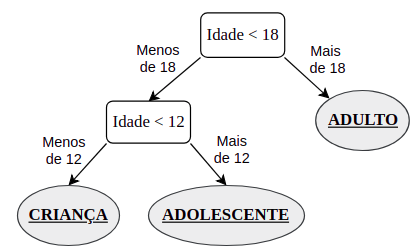
\includegraphics[width=0.6\textwidth]{./dados/figuras/proposta/arvore-decisao}
    \fonte{Autoria própria}
    \label{fig:arvore-decisao}
\end{figure}
    
\subsection{\textit{Random Forest}}
\label{ssec:randomForest}

O \textit{Random Forest} é uma técnica de aprendizado de máquina utilizada tanto para realizar regressões quanto classificações que utiliza múltiplas árvores de decisão para realizar suas predições.

Ela é considerada uma técnica do tipo \textit{bootstrap aggregation}, comumente chamado de \textit{bagging}. No \textit{bagging} algoritmos mais simples são treinados diversas vezes de forma independente utilizando diferentes subconjuntos de dados, gerados por meio de re-amostragem com reposição em um conjunto de treino inicial.

No caso do \textit{Random Forest}, múltiplas árvores de decisão são treinadas independentemente, tomando como base subconjuntos de treinamento formados a partir dos dados de treinamento inicial. 
E o resultado final do algoritmo é definido com base na agregação dos resultados obtidos para cada uma das árvores de decisão \cite{Liaw2002}.

Para classificação é comum o uso da maioria dos votos como estratégia para a definição da classe a ser retornada como resultado. Já para regressão são utilizadas ferramentas estatísticas, como a média aritmética dos resultados retornados por cada árvore de decisão.

A figura \ref{fig:random-forest} apresenta um exemplo simplificado de uma \textit{random forest} de classificação, nela são treinadas quatro árvores de decisão e o resultado da predição é determinado com base na classe que recebe a maioria dos votos, neste caso a classe C.

 \begin{figure}[!htb]
    \centering
    \caption{Exemplo simplificado de \textit{random forest} utilizada para classificação}
    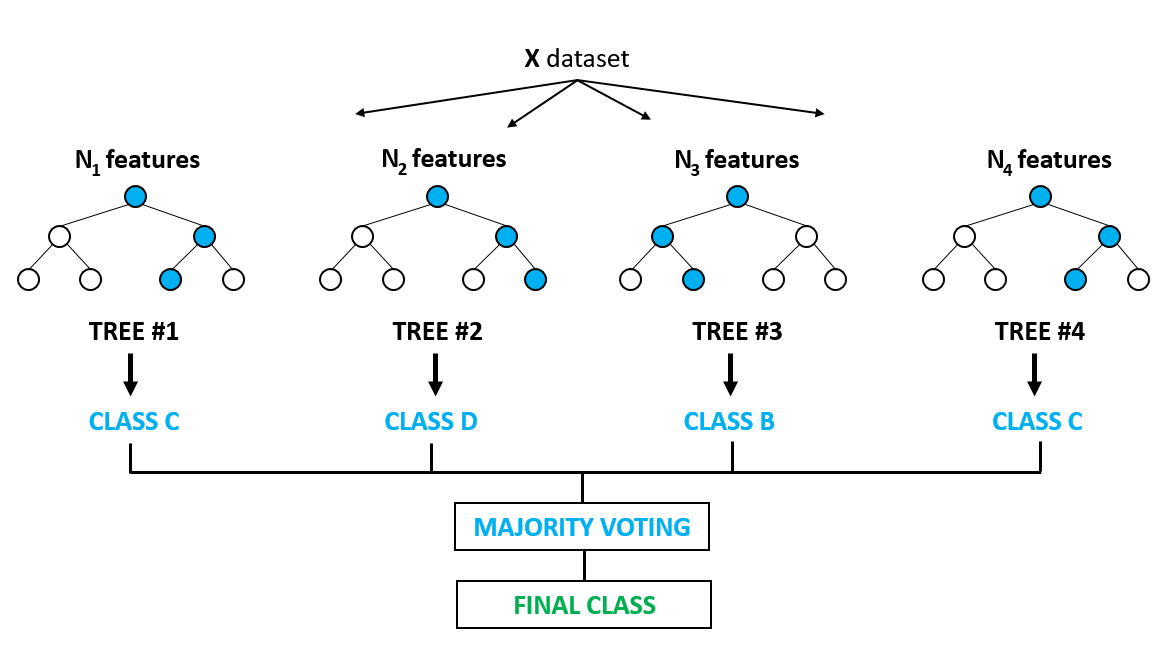
\includegraphics[width=0.8\textwidth]{./dados/figuras/random-forest}
    \fonte{Abilash R. (2018)}
    \label{fig:random-forest}
\end{figure}

\subsection{\textit{Gradient Boosting}}
\label{ssec:gradientBoosting}

Paralelo ao \textit{bagging}, apresentado anteriormente ao descrever o algoritmo \textit{Random Forest}, tem-se os algoritmos do tipo \textit{boosting}.

O princípio dos algoritmos de \textit{boosting} consiste da combinação do resultado de diversos classificadores ou regressores não tão eficientes, a fim de obter um algoritmo final com melhor acurácia. 
Diferente das técnicas de \textit{bagging}, que treinam modelos de forma independente, o \textit{Boosting} treina modelos com base no resultado e no erro de modelos anteriores, encadeando-os. Usualmente os algoritmos de \textit{boosting} utilizam árvores de decisão como algoritmo interno, mas não se limitam a elas \cite{Geron2017}.

Tendo as técnicas de mineração de dados delimitadas, foi-se então definido um modelo metodológico a ser seguido durante o desenvolvimento do trabalho.
A seguir será apresentado o CRISP-DM, modelo utilizado para demarcar as tarefas de um projeto de mineração de dados.

\section{CRISP-DM}
\label{ssec:crisp}
 
O CRISP-DM (\textit{Cross-Industry Standard Process for Data Mining}) é um modelo de processo amplamente utilizado para descrever as etapas da mineração de dados. Um exemplo da aplicação do método é apresentado por \citeonline{Castro2018}, no qual o CRISP-DM é aplicado à um cenário onde é realizado um processo de Busca de Conhecimento em Banco de Dados\footnote{Conhecido também como KDD (\textit{knowledge-discovery in databases}), é o processo de extração de informações valiosas implícitas em bases de dados.} visando a evasão no ensino superior.

O CRISP-DM é composto por seis etapas, que descrevem a sequência de fases para o desenvolvimento de um projeto de mineração de dados. Estas são apresentadas na \autoref{fig:crisp-dm} e são detalhadas a seguir \cite{Chapman2000, Shearer2000}.

\begin{figure}[!htb]
    \centering
    \caption{Método CRISP-DM de modelo de processo para mineração de dados}
    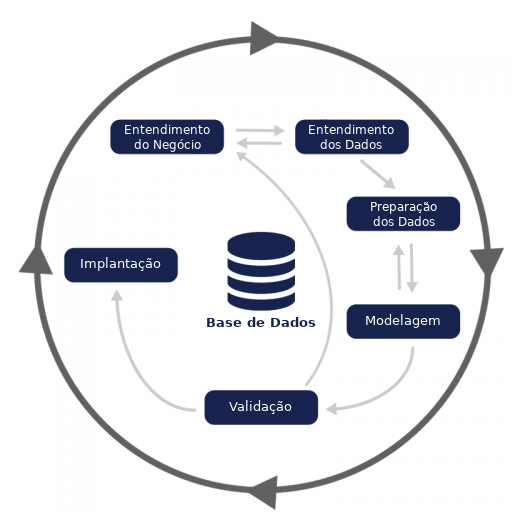
\includegraphics[width=0.6\textwidth]{./dados/figuras/proposta/crisp-dm}
    \fonte{\citeonline{Chapman2000}}
    \label{fig:crisp-dm}
\end{figure}

\subsection{Entendimento do Negócio}

Permite compreender os objetivos do projeto considerando uma perspectiva do negócio, auxiliando na definição do problema de mineração de dados. 
É importante posteriormente para compreender os dados que serão analisados e quais os tipos de valores que se deseja extrair deles.

Pode ser resumido nas seguintes subetapas: definição dos objetivos do negócio, avaliação da situação, definição dos objetivos de mineração de dados e construção do plano de projeto.

\subsection{Entendimento dos Dados}

Esta fase consiste basicamente das seguintes subetapas: coleta inicial dos dados, descrição dos dados, análise dos dados e verificação da qualidade dos dados.
Esta sequência de passos é efetuada de forma que, após a coleta inicial dos dados, objetiva-se desenvolver uma certa familiaridade com os dados, descrevendo-os, para assim identificar problemas de qualidade e subconjuntos de dados que possivelmente contenham informações implícitas.

\subsection{Preparação dos Dados}
\label{sssec:preparacaoDados}

Consiste do tratamento dos dados inicialmente coletados a fim de construir o conjunto final de dados que será utilizado para processamento e análise, e é subdividida em cinco etapas menores: seleção, limpeza, construção, integração e formatação dos dados.

Esta fase se dá inicialmente com a seleção dos dados que serão utilizados para a análise, verificando a sua relevância para os objetivos da mineração de dados, bem como a qualidade e as limitações técnicas quanto ao volume e tipos de dados. 

Após, tem-se a limpeza dos dados, que é responsável por remover dados ruidosos e sem valor para a análise, evitando assim ambiguidades e anomalias nos resultados. 
Nela é feita a conversão de dados que possam estar em um formato não adequado e a remoção de caracteres inválidos, podendo também ser efetuada uma normalização dos dados para ajustá-los à determinadas situações.
Remete a subfase do Entendimento dos Dados, que se refere a verificação da qualidade dos dados. 

Em seguida, na construção dos dados, há a transformação de certos atributos coletados em atributos projetados para facilitar a etapa de processamento, reduzindo em certos casos a quantidade necessária de atributos, como por exemplo ao transformar os atributos \textit{comprimento} e \textit{largura} em somente um atributo \textit{área}. 

Também é importante a integração dos conjuntos de dados coletados relacionando-os para a criação de novos registros, por exemplo quando dois conjuntos de dados possuem valores que podem ser relacionados para gerar dados mais concisos, mas estão fragmentados. 

Por fim tem-se a formatação dos dados, que redesenha o conjunto de dados a fim de permitir sua manipulação por algoritmos e ferramentas específicas.

\subsection{Modelagem}

Nesta etapa do processo são selecionadas técnicas de modelagem de acordo com o problema a ser resolvido. 
Em seguida são gerados testes empíricos para validar a aplicabilidade do modelo, por exemplo a classificação, abordagem supervisionada de aprendizado de máquina utilizada em mineração de dados, utiliza-se taxas de erro entre conjuntos de dados de treinamento e conjuntos de dados de teste para medir sua acurácia. Desta forma verifica-se se o modelo pode prever dados históricos com eficiência, para então utilizá-lo para predizer dados futuros. 

Então o modelo é gerado sobre o conjunto de dados preparados previamente e por fim é realizada a validação do modelo, avaliando a aplicação.

\subsection{Validação}

Nesta fase são avaliados os resultados apresentados pelo modelo, revisando a construção deste se necessário. Valida-se os resultados tomando em conta os objetivos do negócio definidos anteriormente, verificando se todos foram abordados de forma adequada ou se devem ser realizados ajustes nas etapas iniciais do processo. 

Por fim deve-se decidir como utilizar os resultados obtidos com a mineração de dados, caso estes sejam considerados satisfatórios e respondam ao problema de mineração de dados previamente definido.

\subsection{Implementação}

A implementação é a última etapa do CRISP-DM, mas isto não significa que o projeto é finalizado quando atinge esta etapa. 
Como apresentado na \autoref{fig:crisp-dm}, no qual o círculo com as setas mais externas representa a natureza cíclica da mineração de dados, onde se mantém em constante revisão e atualização.

Nesta fase as informações geradas a partir do processamento dos dados são organizadas e apresentadas ao usuário final (e.g. gerentes, analistas, clientes) por meio de gráficos e outras ferramentas de visualização de dados, a fim de auxiliar na análise e assim, nas suas tomadas de decisões.

\section{VISUALIZAÇÃO DE DADOS}

A visualização de dados descreve técnicas que objetiva-se a auxiliar na compreensão e extração de significado de dados utilizando contextos visuais.

Em um conjunto de dados podem haver informações importantes ocultas que podem auxiliar nas tomadas de decisão e a promover negócios.
Mas o desafio é que nem sempre é possível tirar conclusões apenas analisando números brutos.
Quando se analisa os dados apresentados em um formato visual, surgem padrões, conexões e outras descobertas que, de outro modo, não seriam percebidos \cite{Microsoft2018}.

Segundo \citeonline{Cortes2002}, a visualização de dados é extremamente útil como técnica de descobrimento de padrões, e embora possa parecer uma técnica não tão sofisticada, permite mensurar a qualidade inicial dos dados e identificar onde os padrões podem ser extraídos. 

Quando esta é utilizada em processos mais avançados de mineração de dados é possível a criação de gráficos tri-dimensionais interativos e gráficos de segmentação de bancos de dados em forma hierárquica, como uma árvore.

\section{TRABALHOS RELACIONADOS}
\label{sec:trabalhosRelacionados}

A seguir são apresentados trabalhos relacionados que possuem propostas com características semelhantes à deste trabalho.

Em seu trabalho, \citeonline{CorneliusJunior2015} apresenta um estudo sobre a evasão no ensino superior e a aplicação de técnicas de mineração de dados na tentativa de descobrir um perfil dos alunos com tendências evasivas e os padrões associados a essas tendências. 
O autor aplica as técnicas de classificação e associação utilizando a ferramenta de mineração de dados \textit{WEKA}, com base em um conjunto de dados cedidos pela Universidade de Santa Cruz do Sul. 
Neste contexto foram constatados que os fatores que mais influenciaram para a evasão de cursos foram o total de disciplinas cursadas e o status final das disciplinas do primeiro semestre acadêmico. 

\citeonline{Ramos2011} descrevem em seu trabalho uma pesquisa realizada com o objetivo de identificar determinantes para as questões de retenção e evasão no curso de Nutrição da UFRGS. 
Os autores utilizaram diversas abordagens para atingir o maior número de discentes, elaborando questionários eletrônicos para que fosse possível atingir tanto alunos em curso quanto alunos evadidos, e realizando entrevistas com alunos regulares e em situação de retenção. 
Com a conclusão do trabalho os autores explicitam a necessidade de criação de mecanismos de acompanhamento de alunos para a prevenção da retenção e evasão discente, bem como o desenvolvimento de competências relacionadas ao empreendedorismo, como forma de motivação para os alunos.

O trabalho de \citeonline{Marques2015} apresenta um projeto de pesquisa em andamento na área de mineração de dados educacionais, cujo objetivo é a predição do desempenho de estudantes universitários em ambientes convencionais de ensino. 
No trabalho os autores afirmam, que devido ao número elevado e a natureza não linear das variáveis que determinam o desempenho dos estudantes, a previsão pode nem sempre ser satisfatória e os resultados não serem suficientemente bons para tomadas de decisões que ajudem a corrigir os problemas do tema. 
Mas ainda se faz necessária a produção de trabalhos deste cunho, devido a possibilidade de antever, mesmo com certa margem de erro e de tempo, o comportamento de um aluno que se enquadra em um determinado perfil de desempenho, e então motivar o docente responsável pela disciplina a utilizar recursos pedagógicos que busquem recuperar o aluno ainda no tempo regular das aulas da disciplina.

Em um trabalho posterior, \citeonline{Caetano2016} apresenta uma aplicação de técnicas de aprendizado de máquina e mineração de dados com o foco na predição do desempenho acadêmico de alunos. 
Para isto a autora utilizou também o ambiente \textit{WEKA}, empregando três diferentes algoritmos de aprendizado de máquina: o \textit{Naive Bayes}, \textit{Nearest Neighbor} e o J48, versão do WEKA do algoritmo de árvore de decisões C4.5. 
O resultado do seu trabalho mostrou que foi possível prever o desempenho de estudantes com precisão de aproximadamente 70\% utilizando somente informações iniciais e 90\% caso seja utilizado um conjunto de atributos completo ou somente com os atributos mais impactantes para o treinamento do modelo.
Para este trabalho foram utilizados dados demográficos, como sexo, idade e estado civil, e dados associados ao desempenho parcial dos alunos, como notas dos trabalhos entregues durante o periodo letivo.

\citeonline{Rigo2015} apresentam em seu trabalho uma análise de melhorias possíveis na aplicação de mineração de dados educacionais, para que estes possam ser efetivamente utilizados para a detecção de padrões comportamentais relacionados à evasão escolar. 
Os autores salientam a necessidade de mapear os fatores associados ao fenômeno, bem como a necessidade de implantação de soluções interativas, que permitam o acesso dinâmico aos resultados e possibilite o diagnóstico precoce e a realização de ações pedagógicas relevantes para combater à evasão no ensino. 

O modelo proposto por \citeonline{Tinto1987} e posteriormente discutido por \citeonline{Andriola2006} propõe que as características demográficas, como o nível socioeconômico e os conhecimentos adquiridos previamente por meio de educação formal e informal, influenciam na integração do discente com o novo ambiente universitário, e a condição social do discente, como a idade, gênero, habilidades pessoais e expectativas de desenvolvimento pessoal, está fortemente associada com a motivação para o desempenho acadêmico e o seu reconhecimento.

\citeonline{Babosa2017} exploram em seu trabalho aspectos da mineração de dados como recurso tecnológico para investigações em um Ambiente Virtual de Aprendizagem (AVA). 
Com os resultados obtidos os autores indicam que a mineração de dados permite acesso a informações sobre o processo educativo, tais como aproveitamento, desempenho e a predição dos resultados finais, identificando relações entre dados que podem produzir novos conhecimentos. 
Isto permite refletir sobre os métodos de ensino empregados e então tomar decisões para a melhoria do desempenho acadêmico.
\chapter{PLANO DE TRABALHO}
\label{chap:planoTrabalho}

\section{TECNOLOGIAS E FERRAMENTAS}
\label{sec:tecnologiasFerramentas}
Para a implementação do \textit{front-end} do sistema web foi utilizado o framework javascript \textit{React.js}, devido a sua capacidade de construção de \textit{Single Page Applications} (SPAs), que permitem a interação do usuário com as páginas da aplicação sem demandar de recarregamento das páginas.
Nas \textit{SPAs} todo os \textit{templates}, ou seja, códigos \textit{HTML}, \textit{CSS} e \textit{Javascript} dos quais o navegador necessita interpretar para a renderização das páginas, são carregadas no inicio do uso da aplicação, restando somente o carregamento dos dados a serem feitos com as mudanças de telas.

\citeonline{Tesarik2008} mostram em seu trabalho as dificuldades na construção de SPAs por conta do design mais sofisticado que esta deve ter para permitir a movimentação do usuário entre as páginas. 
Mas em contrapartida apresentam uma das principais vantagens deste tipo de construção, que é a melhor fluidez que pode ser obtida na experiência do usuário ao interagir com a aplicação.

Em conjunto ao React.js foram utilizadas as seguintes bibliotecas: 

\begin{itemize}[topsep=5pt]
    \item \textbf{Bootstrap\footnote{Disponível em https://getbootstrap.com/}:} É um pacote de ferramentas para construção do lado do cliente da aplicação, ou seja, o \textit{front-end}. Contém componentes que facilitam a construção e estilização de páginas responsivas, disponibilizando recursos em \textit{HTML}, \textit{CSS} e \textit{Javascript}.  
    \item \textbf{Charts.js\footnote{Disponível em https://chartjs.org/}:} É uma biblioteca rápida, responsiva e flexível utilizada por designers e desenvolvedores para a construção de gráficos.
    \item \textbf{D3.js\footnote{Disponível em https://d3js.org }:} Abreviação para \textit{Data-Driven Documents}, ela é uma biblioteca para criação dinâmica e interativa de gráficos, grafos e outras ferramentas de visualização de dados.
\end{itemize}

Para a implementação do \textit{back-end} foram criados dois programas isolados. 
O primeiro consiste de uma \textit{API} construída utilizando a plataforma Node.js com a linguagem de programação \textit{Typescript}. 
Esta \textit{API} é responsável por dispor todos os dados para as operações que não envolvem predições, ou seja, dados para construção de gráficos e listagem no \textit{front-end}, e também pelo envio de e-mails e preparação dos dados a partir das planilhas carregadas para persistência.
As bibliotecas utilizadas no código em Node.js são:
\begin{itemize}[topsep=5pt]
    \item \textbf{Express\footnote{Disponível em https://expressjs.com/}:} É um framework leve e flexível que possibilita a uma aplicação Node.js criar uma API robusta rapidamente;
    \item \textbf{Mongoose\footnote{Disponível em https://mongoosejs.com/}:} É responsável por mapear os objetos entre o Node.js e o banco de dados MongoDB, gerenciando relacionamentos de dados e provendo a construção de esquemas para validação de regras na inserção de dados, o que garante uma maior consistência dos dados;
    \item \textbf{SheetJS\footnote{Disponível em https://github.com/SheetJS/sheetjs}:} É um plugin leve e robusto para manipulação de planilhas, permitindo a criação, leitura e conversão de planilhas para JSON, entre outros;
    \item \textbf{Moment.js\footnote{Disponível em https://momentjs.com}:} É uma biblioteca que possui um amplo ferramental para manipulação, validação e apresentação de datas em \textit{javascript}, contemplando diferentes fusos horários;
    \item \textbf{Nodemailer\footnote{Disponível em https://nodemailer.com/about/}:} É um modulo gratuito que permite aplicações Node.js realizar o envio de e-mails;
    \item \textbf{SimpleCrypto\footnote{Disponível em https://www.npmjs.com/package/simple-crypto-js}:} Possibilita o processo de encriptação e decriptação por meio de uma chave criptográfica de forma simples.
\end{itemize}

O segundo programa também consiste de uma \textit{API}, desta vez construída utilizando a linguagem de programação Python. 
Esta é responsável pelo treinamento dos modelos de aprendizado de máquina e pelas requisições recebidas do \textit{front-end} relacionadas as predições. 
Para isto são utilizadas algumas bibliotecas. São estas:

\begin{itemize}[topsep=5pt]
    \item \textbf{Flask\footnote{Disponível em https://palletsprojects.com/p/flask/}:} Semelhante ao Express para Python, ele é um módulo leve que disponibiliza toda a estrutura para a criação de uma \textit{API}.
    \item \textbf{PyMongo\footnote{Disponível em https://api.mongodb.com/python/current/}:} É uma biblioteca que dispõe um conjunto de ferramentas para se trabalhar com o MongoDB.
    \item \textbf{NumPy:\footnote{Disponível em https://numpy.org/}} É um pacote de ferramentas matemáticas para computação científica em Python;
    \item \textbf{Pandas\footnote{Disponível em https://pandas.pydata.org/}:} É uma biblioteca \textit{Open-Source} para Python que provêm estruturas de dados e ferramentas de manipulação e análise de dados com alta performance;
    \item \textbf{Matplotlib\footnote{Disponível em https://matplotlib.org/}:} É uma biblioteca para construção de gráficos 2D com poucas linhas de código; 
    \item \textbf{Scikit-learn\footnote{Disponível em https://scikit-learn.org/stable/}:} É uma biblioteca que disponibiliza diversas ferramentas para mineração e análise de dados, como algoritmos de aprendizado de máquina para classificação, regressão e \textit{clusterização}, bem como ferramentas de pré-processamento e validação de modelos.
\end{itemize}

Para persistência foi utilizado o banco de dados não relacional MongoDB.
A escolha do banco de dados (BD) se fez devido a algumas características do modelo não relacional, que permitem uma maior escalabilidade, e mesmo não satisfazendo as propriedades ACID (Atomicidade, Consistência, Isolamento e Durabilidade), que garantem a não duplicidade de dados, é mais flexível e permite estruturar os dados de forma a facilitar a utilização para a geração de gráficos.

O estudo apresentado por \citeonline{Thiago2017}, que compara o MongoDB com o PostgreSQL, sistema de gerenciamento de banco de dados relacional (SGBD), mostra uma maior performance do primeiro BD para a maioria dos casos testados. 

Considerando o cenário de dados acadêmicos, o volume de dados pode se tornar consideravelmente grande, bem como a variedade de dados, desta forma a performance é essencial para a escalabilidade do sistema. Assumindo o crescimento do volume de dados, pode ser desejável o emprego de ferramentas de \textit{Big Data}, e observando que o modelo não-relacional é bastante utilizado e eficaz para o emprego dessas técnicas, o MongoDB se faz adequado.

Para o desenvolvimento deste trabalho foi utilizado o método CRISP-DM, apresentado na subseção \ref{ssec:crisp}. 
Este processo metodológico é subdividido em seis fases principais, que foram seguidas de forma não linear durante o processo de implementação do projeto, desta forma em diversos momentos fez-se necessário revisitar etapas anteriores.

\section{ENTENDIMENTO DO NEGÓCIO}
\label{sec:entendimentoNegocio2}
No contexto apresentado, no qual a principal intenção era analisar dados e construir modelos que permitissem estimar o desempenho de alunos durante o período letivo e implementar mecanismos que possibilitassem interagir com alunos em situações previstas de retenção objetivando-se a reduzir a retenção acadêmica, o entendimento do negócio se fez definindo objetivos de negócio que permitissem compreender alguns fatores relacionados ao contexto acadêmico. 
Estes objetivos de negócio foram definidos por meio das seguintes questões:

\begin{itemize}[topsep=5pt]
    \item Quais fatores sob o domínio de conhecimento da instituição de ensino influenciam para retenção de alunos?
    \item Como as notas e as frequências parciais de um aluno se relacionam?
    \item A partir das notas e frequências parciais de um aluno, é possível determinar o desempenho final dele?
    \item A partir das notas e frequências parciais de alunos, é possível determinar um comportamento comum que descreva a tendência a retenção?
\end{itemize}

Dentre os fatores sob domínio de conhecimento da Instituição de Ensino tem-se os de cunho acadêmico, como:
as notas das avaliações, as notas de todos os trabalhos e entregas e a frequência parcial do aluno (percentual de frequência durante o semestre letivo).
    
% a complexidade das disciplinas, a quantidade de disciplinas cursadas por semestre e os docentes que ministram as disciplinas cursadas pelo aluno.

Foi-se considerado também o uso da plataforma URI Online Judge \cite{URI}, uma ferramenta on-line utilizada por alguns docentes que lecionam disciplinas de programação. A plataforma URI possibilita que os alunos testem seus conhecimentos resolvendo desafios e suporta diferentes linguagens de programação, como C/C++, Java, Python e PSQL.

Além disso, a plataforma possui uma versão acadêmica, que permite que um professor cadastre os alunos de sua turma, disponibilize listas de exercícios específicos e monitore quais alunos resolveram os exercícios, bem como a quantidade de exercícios que cada aluno resolveu, tentou resolver, ou simplesmente não tentou resolver. 

O \textit{URI Academic} possui parceria com várias instituições nacionais, como a Universidade de São Paulo (USP) e a Universidade Tecnológica Federal do Paraná (UTFPR) e internacionais, como a \textit{Baylor University}, do Texas, Estados Unidos, e a \textit{Universidad Nacional Autónoma de México}, situada na Cidade do México \cite{URIAcademic}.

O formato dos dados retornados pela plataforma URI Online Judge são apresentados na figura \ref{fig:planilha-uri}.

\section{ENTENDIMENTO DOS DADOS}
\label{sec:entendimentoDados2}

Nesta fase foi realizada a coleta dos dados iniciais para validação do sistema proposto. Para a implementação foram disponibilizados pelo professor orientador, de forma anônima. 
Neste trabalho foram utilizados dados de quatro turmas da UTFPR - campus Cornélio Procópio, contemplando dados de notas e faltas de 134 alunos.
Complementar a isto foram utilizadas dez planilhas de exercícios do URI, com aproximadamente sete exercícios cada, totalizando 72 exercícios.

Para a aquisição dos dados por parte do sistema de predição desenvolvido, foi-se criado uma página de upload de dados por meio de planilhas.
Nesta página são aceitas planilhas nos formatos disponibilizados pelo sistema de gestão de aprendizagem Moodle, que contemplam todas as notas parciais de avaliações e atividades realizadas via Moodle, bem como o nome, sobrenome e e-mail de cada aluno. 
Vale ressaltar que os nomes das colunas de notas refletem os nomes designados para as atividades criadas no Moodle. 
Então caso o docente se sinta interessado em utilizar o sistema desenvolvido neste trabalho, é importante realizar algumas adaptações na forma como são denominadas as atividades no Moodle, a fim de evitar trabalhos manuais posteriormente ao carregar os dados.

O formato da planilha de notas disponibilizada atualmente pela plataforma Moodle é semelhante ao apresentado na figura \ref{fig:planilha-notas}.

\begin{figure}[!htb]
    \centering
    \caption{Modelo de planilha com notas exportada pelo Moodle}
    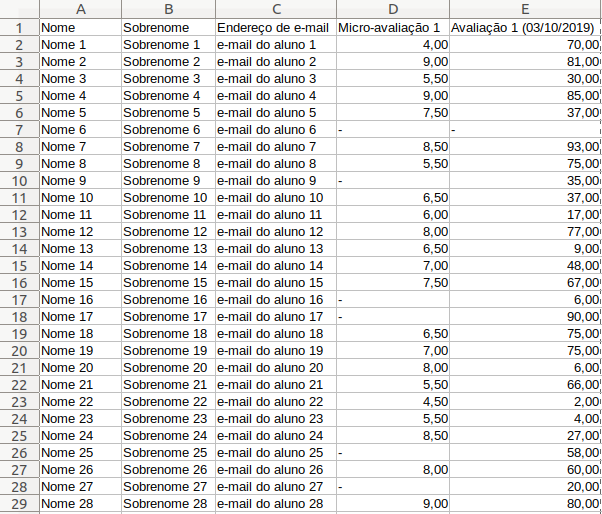
\includegraphics[height=0.6\textwidth]{./dados/figuras/planilha-notas-2}
    \fonte{Autoria Própria}
    \label{fig:planilha-notas}
\end{figure}

Para a submissão das faltas é aceito o formato disponibilizado pelas planilhas exportadas pelo sistema acadêmico da UTFPR. 
Neste arquivo é disposto um código identificador ou Registro Acadêmico (R.A.), nome do aluno, total de faltas e colunas que representam cada um dos dias de aula corridos no período letivo, com o número de ausências de cada aluno em cada um desses dias.

O formato da planilha de faltas disponibilizada atualmente pelo sistema acadêmico da UTFPR é apresentado na figura \ref{fig:planilha-faltas}, mas em alguns casos estas são exportadas com sua estrutura semelhante a apresentada na figura \ref{fig:planilha-faltas-2}. 
A plataforma desenvolvida também está preparada para receber dados neste formato e ao carregar uma planilha neste padrão ele internamente realizará a re-estruturação desta para o formato apresentado na figura \ref{fig:planilha-faltas} e em seguida a extração e persistência dos dados.

\begin{figure}[!htb]
    \centering
    \caption{Modelo de planilha com faltas exportada do sistema acadêmico da UTFPR}
    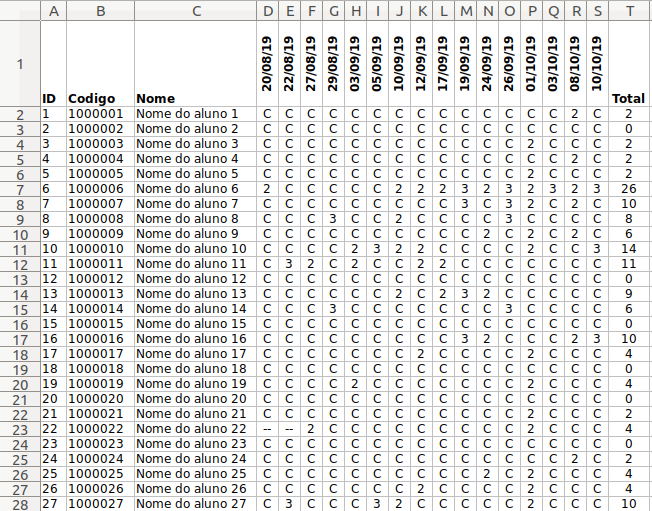
\includegraphics[height=0.6\textwidth]{./dados/figuras/planilha-faltas}
    \fonte{Autoria Própria}
    \label{fig:planilha-faltas}
\end{figure}

\begin{figure}[!htb]
    \centering
    \caption{Modelo alternativo de planilha com faltas exportada pelo sistema acadêmico da UTFPR}
    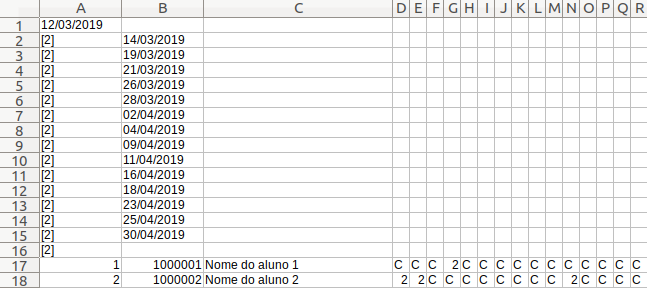
\includegraphics[height=0.35\textwidth]{./dados/figuras/planilha-faltas-2}
    \fonte{Autoria Própria}
    \label{fig:planilha-faltas-2}
\end{figure}

Para o upload de dados de notas e faltas, obtidos no Moodle e sistema acadêmico, respectivamente, é necessário que ambas as planilhas estejam consolidadas em somente um arquivo, como abas, como apresentado na figura \ref{fig:planilha-abas-selecionadas}.
Por mais que reflita em uma etapa a mais de trabalho manual demandado do usuário, isto é usado como um recurso para evitar o upload de notas e de faltas de períodos divergentes ou planilhas que não estão sincronizadas entre si quanto a data corrente do periodo letivo. 
Por exemplo o upload de notas dos alunos até certa data do período letivo e ao mesmo tempo upload das faltas referentes a uma data posterior.

Os nomes das abas não influenciam na importação dos dados, contanto que a ordem delas seja a mesma da apresentada na figura \ref{fig:planilha-abas-selecionadas}, sendo a primeira aba destinada às notas e a segunda aba destinada às faltas dos alunos.

\begin{figure}
\centering
\caption{Planilha de dados com notas e faltas separadas por abas}
\begin{subfigure}{.4\textwidth}
  \centering
  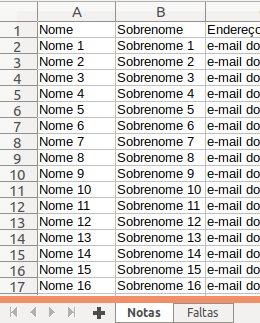
\includegraphics[width=.9\linewidth]{./dados/figuras/planilha-selecionado-notas}
  \end{subfigure}%
\begin{subfigure}{.4\textwidth}
  \centering
  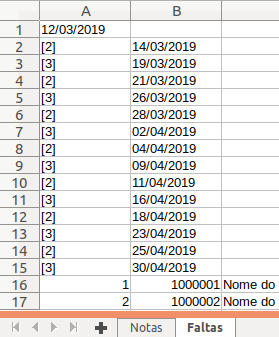
\includegraphics[width=.9\linewidth]{./dados/figuras/planilha-selecionado-faltas}
\end{subfigure}
\label{fig:planilha-abas-selecionadas}
\end{figure}

Além destes dois arquivos, foi considerado como fonte de dados a plataforma URI, citada anteriormente na subseção \ref{sec:entendimentoNegocio2}, desta forma o sistema desenvolvido também possibilita o envio de planilhas com dados da plataforma URI.

\begin{figure}[!htb]
    \centering
    \caption{Modelo de planilha com dados exportada pela plataforma URI}
    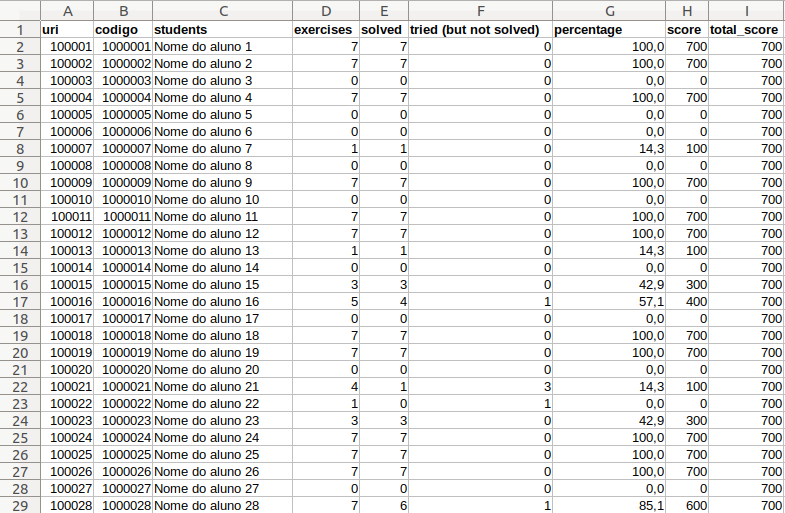
\includegraphics[height=0.6\textwidth]{./dados/figuras/planilha-uri}
    \fonte{Autoria Própria}
    \label{fig:planilha-uri}
\end{figure}

O sistema foi configurado para permitir o upload de arquivos gerados com extensão \textit{xls} e \textit{xlsx}, formatos padrões utilizados pelo gerenciador de planilhas \textit{Excel}, da Microsoft, \textit{ods}, formato utilizado pelo software open-source \textit{LibreOffice Calc}, e \textit{csv}, formato bastante utilizado por sistemas de exportação de texto formatado por vírgulas.

A plataforma também é capaz de distinguir os nomes das colunas, então é recomendado que estes sejam descritos conforme os apresentados nas figuras \ref{fig:planilha-notas}, \ref{fig:planilha-faltas} (caso possível) ou \ref{fig:planilha-faltas-2} e \ref{fig:planilha-uri}. 
Algumas alternativas de nomes de colunas também podem ser utilizadas, como Trabalho 1 ou Atividade 1 ao invés de Micro-avaliação 1, e Prova 1 ao invés de Avaliação 1. 
É importante a inserção das datas das avaliações em seu nome na atividade do Moodle, por exemplo Avaliação 1 - 03/10/2019 ou Avaliação 1 (03/10/19), para que seja possível associar as faltas até esta data. 
Não é necessário seguir um padrão específico de separador entre o nome da atividade e a data, uma vez que é utilizado uma expressão regular para capturar a data no título, caso existente.

Lembrando que todas as planilhas citadas anteriormente são disponibilizadas pelos seus respectivos sistemas, assim a coleta destes e inserção no sistema de predição ainda é feita de forma manual, mas o trabalho manual de manipulação dos dados das planilhas é eliminado.

Após a aquisição dos dados iniciais, que foram utilizados para estruturar a aplicação, foi-se identifica a relação entre os tipos de planilhas inseridos por meio do código identificador do aluno.
Foi possível verificar também que a planilha de notas pode contém valores faltantes, campos vazios ou com caracteres especiais como o ``-'' (traço). 
Analisando-o pode-se perceber que estes pertencem a alunos que não realizaram provas ou atividades, e estes podem ser substituídos por um valor padrão, neste caso o valor 0 (zero).

Foi-se então realizada uma análise dos dados, considerando a princípio as notas das avaliações, a realização de trabalho, a resolução de exercícios do URI e as frequências dos alunos. 
Com isto gerou-se alguns gráficos.

A figura \ref{fig:analise-1} mostra um gráfico de dispersão contendo no eixo horizontal as frequências dos alunos e no eixo vertical a nota média destes. 
Usou como variável também a realização ou não de trabalhos, os pequenos círculos ilustram os alunos que deixaram de realizar algum dos trabalhos, enquanto que os símbolos em X ilustram os alunos que realizaram todas as atividades. 
Pode-se perceber uma concentração de maiores notas quando os alunos possuem maiores frequências nas aulas e a realização dos trabalhos propostos torna ainda mais evidente esta relação.

\begin{figure}[!htb]
    \centering
    \caption{Gráfico de dispersão com as frequências e notas dos alunos, considerando a realização de todos os trabalhos}
    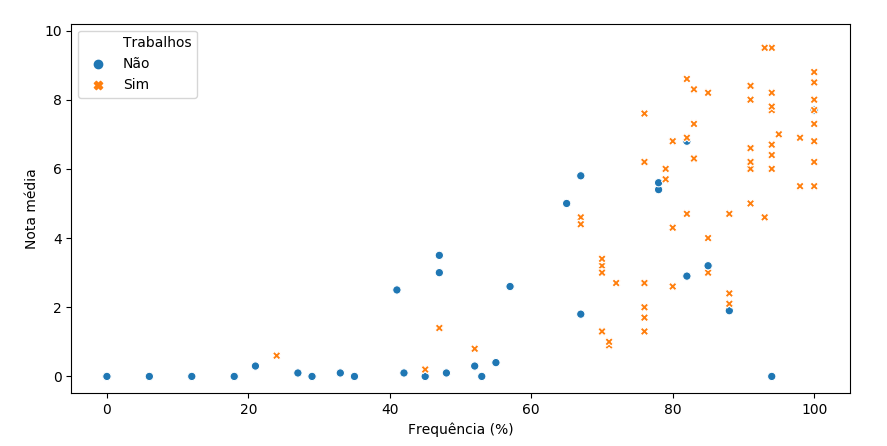
\includegraphics[width=1\textwidth]{./dados/figuras/analise/grafico1}
    \fonte{Autoria Própria}
    \label{fig:analise-1}
\end{figure}

A figura \ref{fig:analise-2} apresenta um gráfico com dois \textit{subplots}, no eixo horizontal de ambos é apresentado a nota obtida, já o eixo vertical mostra a quantidade de alunos com esta nota.
O \textit{plot} da esquerda é composto pelos alunos que realizaram todos os trabalhos e o da direita pelos alunos que não realizaram algum dos trabalhos. 
Pode-se observar uma maior concentração de alunos com boas notas na ilustração da esquerda, já no da direita a distribuição das notas diferente, não havendo notas maiores do que oito. 
Neste o número de alunos com nota zero ultrapassa oito, mas para melhor comparação foi-se limitado o eixo vertical de ambos os gráficos neste valor.

\begin{figure}[!htb]
    \centering
    \caption{Gráficos de barra com as quantidades de alunos por faixa de notas}
    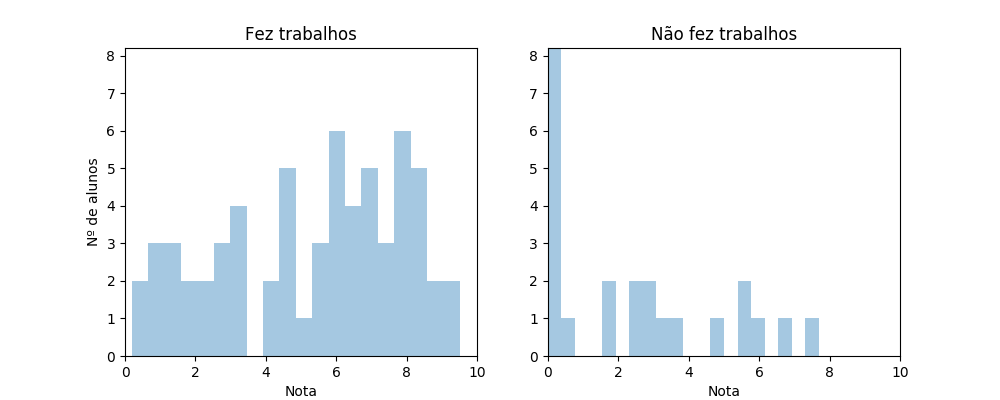
\includegraphics[width=1\textwidth]{./dados/figuras/analise/grafico2}
    \fonte{Autoria Própria}
    \label{fig:analise-2}
\end{figure}

Já as figuras \ref{fig:analise-3} e \ref{fig:analise-4} mostram as notas e o número de alunos mas segmentando-as pela resolução dos exercícios do URI. 
Para ambas, a ilustração da esquerda mostra os alunos que resolveram 50\% ou mais dos exercícios propostos, enquanto nos gráficos da direita é descrito os alunos que resolveram menos de 50\% dos exercícios.
Ao averiguá-los é possível perceber que a realização dos trabalhos em conjunto da resolução dos exercícios do URI foi o padrão seguido que apresentou melhores resultados, neste a distribuição das notas ficou mais concentrada entre 5,5 e 9,5.

Em contrapartida, para os alunos que não realizaram trabalhos nem exercícios do URI a concentração se deu entre 0 e 0,5, neste também o gráfico foi limitado ao valor cinco, mas a quantidade real de alunos com nota zero foi 16.

Para a concepção destes gráficos foram utilizados os dados de todos os alunos e então é importante observar que há a possibilidade de que uma parcela considerável das notas mais baixas seja referente a alunos que nunca compareceram as aulas ou em pouco tempo deixaram de frequentá-las.

\begin{figure}[!htb]
    \centering
    \caption{Gráficos de barra com as quantidades de alunos que realizaram todos os trabalhos por faixa de notas, considerando os exercícios do URI}
    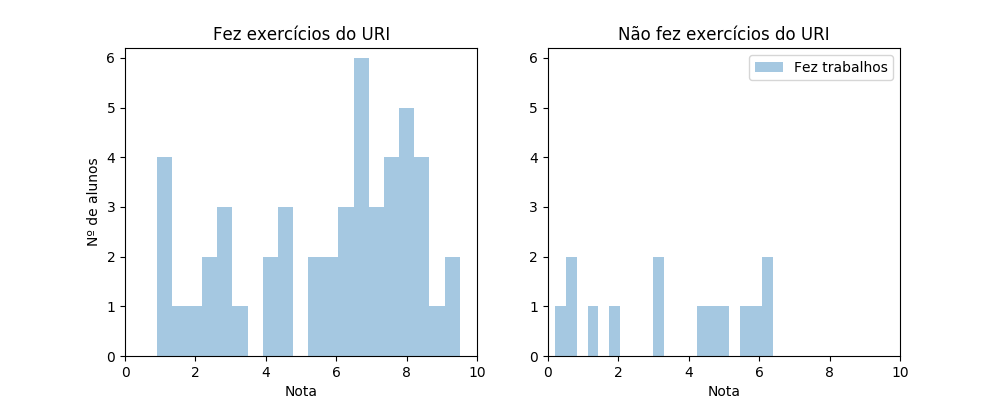
\includegraphics[width=1\textwidth]{./dados/figuras/analise/grafico3}
    \fonte{Autoria Própria}
    \label{fig:analise-3}
\end{figure}

\begin{figure}[!htb]
    \centering
    \caption{Gráficos de barra com as quantidades de alunos que deixaram de realizar algum trabalho por faixa de notas, considerando os exercícios do URI}
    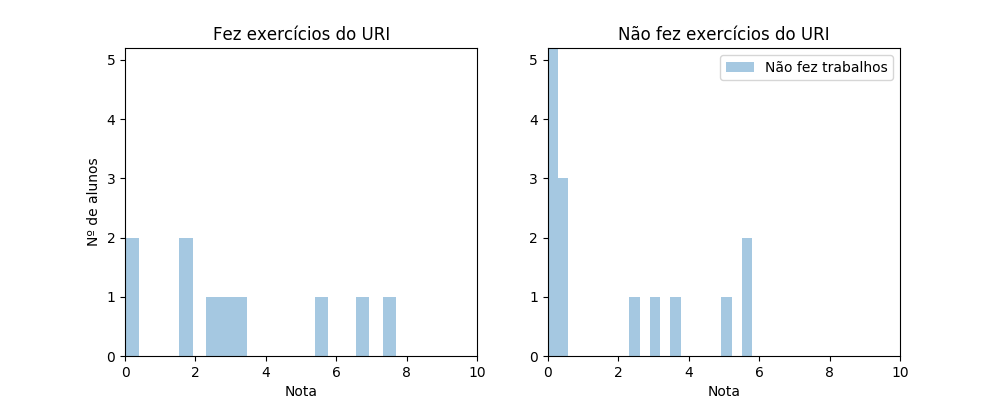
\includegraphics[width=1\textwidth]{./dados/figuras/analise/grafico4}
    \fonte{Autoria Própria}
    \label{fig:analise-4}
\end{figure}


\section{PREPARAÇÃO DOS DADOS}

Como já descrito no tópico \ref{sssec:preparacaoDados}, esta etapa consiste em tratar os dados a fim de dispor o conjunto de dados que será utilizado para o processamento e construção do modelo de mineração de dados, bem como para outros fins, como para apresentação e construção dos gráficos.

Nesta fase foram criados \textit{scripts} para formatação dos dados, a fim de permitir o uso destes para o processamento sem ruídos, incoerências ou redundâncias, reduzindo assim as chances de resultados anômalos.

Inicialmente implementou-se um \textit{script} no \textit{back-end} em Node.js, que efetua a formatação dos dados iniciais para um formato mais adequado para a construção de gráficos e uso nos modelos de predição.
Neste \textit{script} os dados das planilhas são convertidos para o formato JSON utilizando a biblioteca \textit{SheetJS}, que torna mais simples a manipulação dos dados, já que o formato é nativo o linguagem de programação \textit{Typescript}, utilizada no projeto.
Em seguida as notas e frequências inicialmente armazenadas em tipo texto são convertidas para valores numéricos, e as letras que eram utilizadas para representar o status de presença do aluno foram convertidas também para valores numéricos.
Neste contexto a letra C representa os alunos presentes e a letra D representam que este havia sido dispensado com alguma justificativa, como a participação em algum evento ocorrente na universidade, e por isso não havia a contagem de faltas.

Como pode-se observar, as etapas do modelo CRISP-DM são nitidamente conectadas, visto que este último tratamento citado envolve também a etapa de entendimento dos dados. 

A figura \ref{fig:dados-notas-pos} apresenta a estrutura final dos dados de notas, que compõe além das notas alguns outros dados essenciais para o trabalho, que serão melhor detalhados posteriormente. 
A estrutura dos dados é composta pelos seguintes campos:

\begin{itemize}[topsep=5pt]
    \item \textbf{\_id:} ID de Objeto único gerado para este documento pelo MongoDB, ou seja, é a chave primária deste registro no banco de dados;
    \item \textbf{code:} Código identificador/R.A. do aluno;
    \item \textbf{course\_unit:} Código da disciplina ao qual o aluno está vinculado e as notas são referentes;
    \item \textbf{name:} Contém o nome completo do aluno;
    \item \textbf{email:} Campo que contém o e-mail do aluno;
    \item \textbf{attendance:} Contém a frequência, em percentual, do aluno para a disciplina associada a este registro, é calculada com base na quantidade de aulas dadas;
    \item \textbf{current\_grade:} Contém a nota atual do aluno, é calculada com base no peso aplicado para avaliações e atividades;
    \item \textbf{feedbacks:} Este campo é destinado a conter a lista de notificações enviadas por e-mail ao aluno pela plataforma, juntamente às justificativas, ou \textit{feedbacks}, enviados pelo aluno para cada e-mail recebido.
\end{itemize}

Os campos a seguir são gerados dinamicamente conforme as colunas existentes na planilha origem do dado, podendo assim haver um ou mais campos para notas de avaliação, gerando assim campos \textit{gradeN}, sendo N o número de cada avaliação.
Bem como é possível não haver campos para datas de prova, caso esta não esteja presente no cabeçalho da coluna na planilha.
A mesma lógica se aplica para as atividades, podendo assim haver zero, uma ou múltiplas atividades realizadas pelo aluno.

\begin{itemize}[topsep=5pt]
    \item \textbf{grade1:} Contém a nota obtida pelo aluno para a 1ª avaliação da disciplina associada a este registro;
    \item \textbf{grade1\_date:} Contém a data da 1ª avaliação;
    \item \textbf{micro\_grade1:} Contém a nota obtida pelo aluno para a 1ª atividade realizada na disciplina.
\end{itemize}

\begin{figure}[!htb]
    \centering
    \caption{Fragmento do conjunto de dados de notas após preparação}
    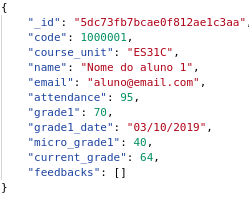
\includegraphics[height=0.35\textwidth]{./dados/figuras/dados-notas-pos}
    \fonte{Autoria Própria}
    \label{fig:dados-notas-pos}
\end{figure}

Então as faltas, que são apresentadas por aula dada, são transformadas para um formato acumulativo, o que facilita também a construção dos gráficos.
Todas estas transformações são realizadas sobre dados no formato apresentado anteriormente na figura \ref{fig:planilha-faltas}, e o resultado é apresentado na figura \ref{fig:dados-faltas-pos}, que exibe o conjunto de dados pós-preparação.

Por fim os dados são armazenados no banco de dados com o uso do \textit{Mongoose}, e a figura \ref{fig:dados-faltas-pos} mostra a estrutura de dados JSON no formato final, que é composta pelos seguintes campos:

\begin{itemize}[topsep=5pt]
    \item \textbf{\_id:} ID de Objeto único gerado para este documento pelo MongoDB, ou seja, é a chave primária deste registro no banco de dados;
    \item \textbf{code:} Código identificador/R.A. do aluno; 
    \item \textbf{course\_unit:} Código da disciplina ao qual o aluno está vinculado e as faltas são referentes;  
    \item \textbf{active:} Campo booleano utilizado para definir o status do aluno na disciplina, caso a frequência seja verificada abaixo de 25\% do total de aulas o aluno é considerado inativo, caso contrário é ativo;
    \item \textbf{total:} Contém o número total de faltas do aluno para a disciplina relacionada no momento do upload dos dados; 
    \item \textbf{absences:} É um campo do tipo Array, que contém um objeto para cada dia de aula dada até o momento. Os campos de cada objeto representam a data da aula e o número de faltas acumuladas do aluno ao decorrer das aulas.
    \item \textbf{id:} Campo opcional, é populado caso a planilha carregada possua uma coluna nomeada como ID e é utilizado para ordenação.
\end{itemize}

\begin{figure}[!htb]
    \centering
    \caption{Fragmento do conjunto de dados de faltas após preparação}
    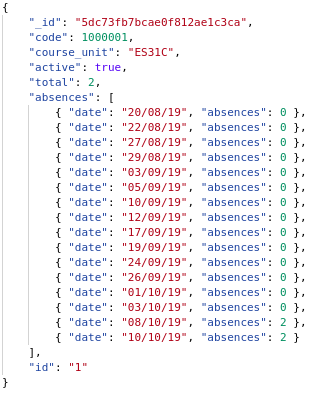
\includegraphics[height=0.65\textwidth]{./dados/figuras/dados-faltas-pos}
    \fonte{Autoria Própria}
    \label{fig:dados-faltas-pos}
\end{figure}

A figura \ref{fig:dados-uri-pos} mostra parcela dos dados após a preparação realizada ao receber a planilha de dados exportada pela plataforma URI.
Estes são compostos pelos seguintes campos:

\begin{itemize}[topsep=5pt]
    \item \textbf{\_id:} ID de Objeto único gerado para este documento pelo MongoDB, ou seja, é a chave primária deste registro no banco de dados;
    \item \textbf{code:} Código identificador/R.A. do aluno; 
    \item \textbf{course\_unit:} Código da disciplina ao qual o aluno está vinculado e os exercicios do URI são referentes; 
    \item \textbf{name:} Contém o nome completo do aluno;
    \item \textbf{exercises:} Contém a quantidade de exercícios aos quais o aluno solucionou completa ou parcialmente;
    \item \textbf{solved:} Contém a quantidade de exercícios que o aluno finalizou corretamente;
    \item \textbf{tried:} Contém a quantidade de exercícios que o aluno tentou solucionar, mas não os finalizou;
    \item \textbf{percentage:} Contém a porcentagem de exercícios solucionados de forma integral;
    \item \textbf{total:} Contém a quantidade total de exercícios para a lista em questão;
    \item \textbf{exam:} Contém a referência da avaliação a qual este registro é associado.
\end{itemize}

\begin{figure}[!htb]
    \centering
    \caption{Fragmento do conjunto de dados obtidos na plataforma URI após preparação}
    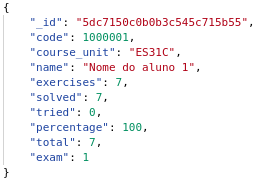
\includegraphics[height=0.32\textwidth]{./dados/figuras/dados-uri-pos}
    \fonte{Autoria Própria}
    \label{fig:dados-uri-pos}
\end{figure}

Vale ressaltar que para um volume pequeno de dados, estas alterações poderiam ser efetuadas manualmente sem grande demanda de tempo, mas para um volume maior de dados, como possivelmente esperado no uso da plataforma desenvolvida, se faz necessário a criação de rotinas de preparação de dados para a realização destas tarefas.
Ressalta-se também que este trabalho tem como objetivo automatizar o maior número possível de tarefas, demandando o mínimo de atuação manual por conta do usuário após a aquisição dos dados.

\section{MODELAGEM}
\label{sec:modelagem}
Uma vez realizada a preparação dos dados, é possível seguir para a implementação dos modelos de mineração de dados.

Neste trabalho foram utilizados três algoritmos de \textit{machine learning} (ML), ou aprendizado de máquina supervisionados, são estes a regressão linear, o \textit{random forest} e o \textit{gradient boosting}, descritos na seção \ref{sec:mineracaoDados}, que descreve a mineração de dados.
Como um dos objetivos deste trabalho é predizer o desempenho dos alunos com base em suas notas e faltas, os algoritmos foram utilizados como técnicas de regressão, mesmo o \textit{random forest} e o \textit{gradient boosting} possuindo a capacidade de atuar como técnicas de classificação de dados.

Desta forma foram implementados os algoritmos com o auxílio das bibliotecas de aprendizado de máquina \textit{Scikit-Learn} e de manipulação de dados \textit{Pandas}.

O trecho de código apresentado na listagem \ref{cod:treinamentoModelos} é utilizado para treinar os modelos de ML citados.
O conjunto de dados foi dividido em subconjuntos de treinamento e teste utilizando a razão 80\%/20\%.
O modelo baseado em \textit{Gradient Boosting} foi gerado com 400 estimadores, que internamente se traduzem em árvores de regressão em formato \textit{boosting}, descrito na \ref{ssec:gradientBoosting}, com profundidade máxima igual a cinco e empregando a função erro \textit{least squares}, ou mínimos quadrados.
O modelo que utiliza \textit{Random Forest} foi gerado utilizando também 400 estimadores, que desta vez geram árvores de regressão em formato \textit{bagging}, descrito na \ref{ssec:randomForest}.
Já o algoritmo de regressão linear não demanda nenhum argumento específico para a criação e treinamento de modelos.

\begin{lstlisting}[caption={Trecho de código para treinamento dos modelos de ML}, label={cod:treinamentoModelos}]

## Divisao do conjunto de dados em treinamento (80%) e teste (20%).
x_train, x_test, y_train, y_test = train_test_split(data.values, labels.values, test_size=0.2, random_state=42)

## Gradient Boosting Model
gradient_model = GradientBoostingRegressor(n_estimators=400, max_depth=5, loss='ls')
gradient_model.fit(x_train, y_train)

## Random Forest Model
random_forest = RandomForestRegressor(n_estimators=400)
random_forest.fit(x_train, y_train)

## Linear Regression Model
linear_regression = LinearRegression()
linear_regression.fit(x_train, y_train)
\end{lstlisting}

A biblioteca \textit{Scikit-learn} possibilita extrair a importância, ou peso, de cada \textit{feature} dos modelos treinados com os algoritmos \textit{Gradient Boosting} e \textit{Random Forest}, ou seja, é possível obter a porcentagem que cada variável utilizada no treinamento influencia nas estimativas retornadas pelos modelos.
A tabela \ref{tab:importanciaGradient} mostra a importância das \textit{features} no modelo treinado com o algoritmo \textit{Gradient Boosting}, considerando dados de turmas que realizaram duas avaliações e três atividades/trabalhos.
A tabela \ref{tab:importanciaRandom} também apresenta a importância das \textit{features}, entretanto para o modelo treinado com o algoritmo \textit{Random Forest}.

\begin{table}[!htb]
    \centering
    \caption{Importância das \textit{features} para o modelo treinado com \textit{Gradient Boosting}}
    \begin{tabular}{@{}cc@{}}
        \hline
        \textbf{ Feature } & \textbf{ Importância } \\ \hline
        grade2  & 79,7\% \\
        micro\_grade1  & 8,9\% \\
        grade1  & 7,8\% \\
        attendance  & 3,2\% \\
        micro\_grade3  & 0,4\% \\
        micro\_grade2  & 0,0\% \\ \bottomrule
    \end{tabular}
    \label{tab:importanciaGradient}
\end{table}

\begin{table}[!htb]
    \centering
    \caption{Importância das \textit{features} para o modelo treinado com \textit{Random Forest}.}
    \begin{tabular}{@{}cc@{}}
        \hline
        \textbf{ Feature } & \textbf{ Importância } \\ \hline
        grade2  & 55,7\% \\
        grade1  & 22,3\% \\
        attendance  & 14,5\% \\
        micro\_grade1  & 5,2\% \\
        micro\_grade3  & 1,7\% \\
        micro\_grade2  & 0,6\% \\ \bottomrule
    \end{tabular}
    \label{tab:importanciaRandom}
\end{table}

Já a tabela \ref{tab:importanciaUmaProva} apresenta os pesos das \textit{features} para ambos os modelos considerando somente uma avaliação e uma atividade/trabalho, mas com atividades da plataforma URI realizadas pela turma, o campo \textit{percentage} no treinamento do modelo contém a porcentagem de exercícios solucionados ou que houve tentativa de resolução pelo aluno.
Desta forma as únicas \textit{features} disponíveis para a criação do modelo foram a nota da avaliação, a nota da atividade e a frequência do aluno.

\begin{table}[!htb]
    \centering
    \caption{Importância das \textit{features}, considerando somente uma avaliação e um trabalho, para modelos treinados com \textit{Gradient Boosting} e \textit{Random Forest}.}
    \begin{tabular}{@{}ccc@{}}
    \textbf{} & \multicolumn{2}{c}{\textbf{Importância}} \\ \midrule
    \textbf{Feature} & \textbf{Gradient B.} & \textbf{Random F.} \\ \midrule
        grade1  & 89,6\%  & 92,7\% \\
        micro\_grade1  & 8,2\%  & 5,1\% \\
        attendance  & 1,2\%  & 1,1\% \\ 
        percentage  & 1,0\%  & 1,1\% \\ \bottomrule
    \end{tabular}
    \label{tab:importanciaUmaProva}
\end{table}

Como apresentado na \ref{sec:entendimentoDados2}, ao realizar o upload da planilha de faltas são salvas também as presenças dos alunos a cada aula dada no período letivo. então construiu-se modelos com base nos dois algoritmos utilizados anteriormente considerando as datas de cada aula, a fim de avaliar a importância individual das aulas nas predições. 
A tabela \ref{tab:importanciaComDatas} apresenta os pesos retornados pelos dois modelos, nesta as datas são representadas pelos campos date\_N, onde N é sequencialmente o número da aula dada. 
A título de exemplificação, ao realizar um paralelo com os dados já apresentados nas seções de entendimento e preparação dos dados, os campos \textit{date\_1} e \textit{date\_2} da tabela \ref{tab:importanciaComDatas} remetem respectivamente às datas 20/08/19 e 22/08/19 da figura \ref{fig:dados-faltas-pos}, e assim sucessivamente.

\begin{table}[!htb]
    \centering
    \caption{Importância das \textit{features}, considerando datas, para os modelos treinados com \textit{Gradient Boosting} e \textit{Random Forest}.}
    \begin{tabular}{@{}ccc@{}}
    % \cmidrule(l){2-3}
    \textbf{} & \multicolumn{2}{c}{\textbf{Importância}} \\ \midrule
    \textbf{Feature} & \textbf{Gradient B.} & \textbf{Random F.} \\ \midrule
        grade1 & 89,7\%  &  91,3\% \\
        micro\_grade1  & 8,4\%  &  7,6\% \\
        attendance  & 0,8\%  &  1,0\% \\
        date\_13  & 0,2\%  &  0,1\% \\
        date\_12  & 0,2\%  &  0,1\% \\ 
        date\_11  & 0,1\%  &  0,0\% \\
        date\_8  & 0,1\%  &  0,0\% \\
        date\_7  & 0,1\%  &  0,0\% \\
        date\_5  & 0,1\%  &  0,0\% \\
        date\_2  & 0,1\%  &  0,0\% \\
        date\_6  & 0,0\%  &  0,0\% \\
        date\_4  & 0,0\%  &  0,0\% \\
        date\_9  & 0,0\%  &  0,0\% \\
        date\_10  & 0,0\%  &  0,0\% \\
        date\_3  & 0,0\%  &  0,0\% \\
        date\_1  & 0,0\%  &  0,0\% \\
        date\_14  & 0,0\%  &  0,0\% \\
        date\_15  & 0,0\%  &  0,0\% \\
        \bottomrule
    \end{tabular}
    \label{tab:importanciaComDatas}
\end{table}

O algoritmo de regressão linear não possui o artificio de identificação das importâncias como os outros, porém ele permite obter os coeficientes determinados pelo modelo para a composição da equação linear que descreve os dados.
Estes coeficientes considerando o conjunto de dados com duas avaliações são apresentados na tabela \ref{tab:coef-linear}.

\begin{table}[!htb]
    \centering
    \caption{Coeficientes definidos pelo modelo de regressão linear considerando duas avaliações}
    \begin{tabular}{@{}cc@{}}
        \hline
        \textbf{ Feature } & \textbf{ Coeficiente } \\ \hline
        grade2  & 0,473 \\
        grade1  & 0,407 \\
        micro\_grade1  & 0,048 \\
        micro\_grade3  & 0,041 \\
        micro\_grade2  & 0,027 \\
        attendance  & 0,008 \\
        percentage  & -0,004 \\ \bottomrule
    \end{tabular}
    \label{tab:coef-linear}
\end{table}

% Ao final será verificado se às questões construídas na subseção \ref{sec:entendimentoNegocio2} podem ser respondidas e se os resultados são satisfatórios. Se forem, estes podem ser levados à etapa de implantação.

\section{IMPLEMENTAÇÃO}
\label{sec:implementacao}

Para esta etapa do trabalho, foi-se então construído um sistema web, do qual tem como finalizar permitir o acesso aos dados, gráficos e artifícios implementados.
O sistema é composto por seis páginas, sendo que quatro destas estão dispostas no menu lateral da plataforma, são estas: \textbf{Dashboard}, \textbf{Configurações}, \textbf{Upload de Dados},  e \textbf{Lista}.
A quinta página é a de \textbf{Detalhes do Estudante} e pode ser acessada pelo Dashboard ou pela Lista ao clicar em uma das linhas das listas de alunos. 
E a última página é a página de \textbf{Feedback} acessada somente pelos alunos por meio de um link exclusivo. Este recurso será melhor explorado posteriormente.

A figura \ref{fig:diagrama-1} apresenta as chamadas realizadas entre os componentes do sistema quando realizado o upload de uma planilha. 
Inicialmente o usuário carrega a planilha por meio da página de upload de dados do sistema, essa é enviada ao \textit{back-end} escrito em Node.js, que por sua vez realiza a manipulação das planilhas, transformação em formato JSON e a preparação dos dados. 
Em seguida os dados formatados são inseridos na base de dados MongoDB com auxílio do \textit{Mongoose}.

\begin{figure}[htb]
    \centering
    \caption{Fluxo de interações entre os componentes do sistema no upload de dados}
    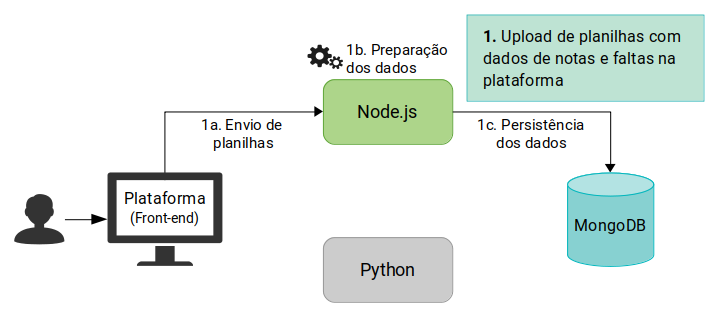
\includegraphics[height=0.35\textwidth]{./dados/figuras/diagrama1}
    \fonte{Autoria Própria}
    \label{fig:diagrama-1}
\end{figure}

Já para chamadas requisitando dados, a figura \ref{fig:diagrama-2} ilustra o processo, que pode ser realizado por dois caminhos distintos:

\begin{enumerate}[topsep=5pt]
    \item \textbf{Dados em geral:} Estes são utilizados para apresentação, listagem ou para construção de gráficos no \textit{front-end}, e para este tipo de dados são realizadas chamadas ao \textit{back-end} Node.js, que busca os dados no BD, transforma-os conforme a demanda específica, realiza os cálculos necessários para apresentação, como a média de faltas da turma para cada aula do período letivo e a média das notas dos alunos em cada disciplina, e então retorna-os.
    \item \textbf{Predições:} Para predições a chamada é enviada para o \textit{back-end} em Python, que busca os dados necessários no BD, reformata-os para o uso com os modelos de machine learning criados e citados anteriormente, busca o modelo correto a ser carregado com base nos dados atuais do aluno e então executa os algoritmos, retornando os resultados. 
\end{enumerate}

\begin{figure}[!htb]
    \centering
    \caption{Fluxo de interações entre os componentes do sistema em requisições solicitando dados e predições}
    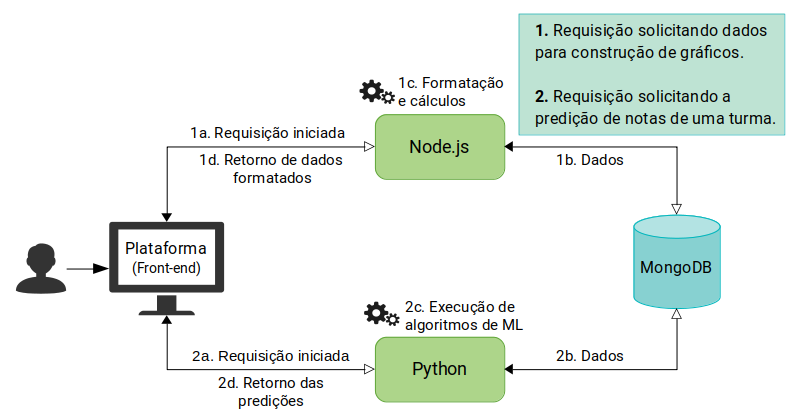
\includegraphics[height=0.45\textwidth]{./dados/figuras/diagrama2}
    \fonte{Autoria Própria}
    \label{fig:diagrama-2}
\end{figure}

\subsection{Dashboard}
\label{ssec:dashboard}

A página inicial da plataforma consiste do Dashboard. 
Este é apresentado nas figuras \ref{fig:dashboard-1} e \ref{fig:dashboard-2}.
Os indicadores apresentados no topo nas cores verde, amarelo e vermelho levam em conta a nota dos alunos e mostram o número de alunos em situações tendenciosas a aprovação, com notas medianas e com um risco maior de reprovação, respectivamente.
Para esta separação foram criados dois \textit{thresholds} e com base em um sistema de notas de 0 a 100 foram sugeridas as seguintes regras:
\begin{itemize}[topsep=5pt]
    \item \textbf{Aprovado:} Nota prevista maior ou igual a 70;
    \item \textbf{Limiar:} Nota prevista entre 50 e 70;
    \item \textbf{Alto risco:} Nota prevista abaixo de 50;
\end{itemize}

Estas regras foram criadas como uma forma de priorização de perfis de alunos na realização de ações, ou seja, os usuários do sistema, interessados em interagir com os alunos ou desenvolver mecanismos para prevenir a retenção podem iniciar com o perfil de \textit{alto risco} como seu público alvo. 
Da mesma pode-se tomar diferentes ações com o perfil \textit{limiar}, uma vez que estes alunos, em tese, demandam de menos esforço para garantir a aprovação nas disciplinas.

Localizados na direita superior da figura \ref{fig:dashboard-1} tem-se o número total de alunos cadastrados na plataforma e uma caixa de seleção flutuante, que permite selecionar uma das disciplinas cadastradas ou manter a opção Todas as Disciplinas para visualizar os dados de forma geral.

Ainda na figura \ref{fig:dashboard-1} tem-se o gráfico temporal de faltas dos alunos de uma turma, comparando-as com o limite parcial para reprovação por faltas da UTFPR, atualmente de 25\% do total de aulas dadas no período letivo.
O eixo horizontal é composto pelas datas dos dias de aula até o momento em que os dados foram carregados na ferramenta, e o eixo vertical mostra a média das ausências absolutas em cada aula dos alunos de uma turma, neste caso da disciplina ES31C - Laboratório de Informática.

Para obter números mais práticos e condizentes com a realidade, no cálculo desta média não são considerados os alunos inativos, ou seja, que possuem menos de 25\% de frequência, pois a inserção de dados de alunos que cancelaram sua matrícula, nunca foram as aulas ou foram somente nas aulas iniciais poderia influenciar negativamente nos números gerais. 
Estes alunos ainda podem ser analisados individualmente, porém para efeitos de cálculos coletivos eles não são considerados.

A escolha do \textit{threshold} para determinar se um aluno é ativo ou inativo foi estipulada de forma empírica observando os dados disponíveis, mas caso seja observado ao longo do tempo um valor mais preciso para descrever esse comportamento, o \textit{threshold} poderia ser alterado.

\begin{figure}[!htb]
    \centering
    \caption{Fragmento superior do dashboard}
    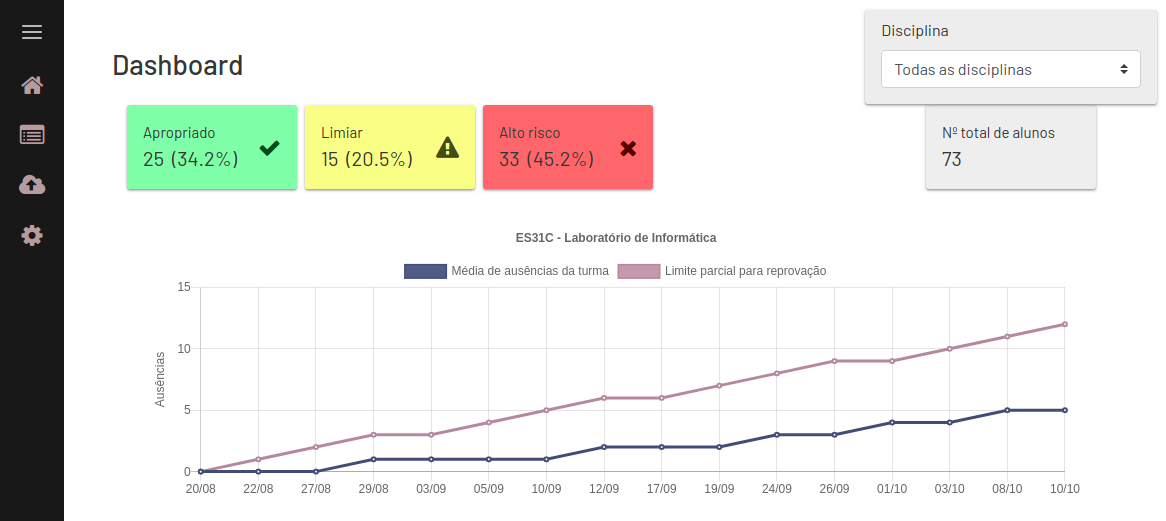
\includegraphics[width=1\textwidth]{./dados/figuras/sistema/sistema-dashboard-1}
    \fonte{Autoria Própria}
    \label{fig:dashboard-1}
\end{figure}

A figura \ref{fig:dashboard-2} apresenta a segunda parte do dashboard. 
O primeiro gráfico apresentado nesta tela tem como objetivo mostrar a relação entre a frequência e notas dos alunos, caso exista, levando em conta se estes realizaram atividades/trabalhos ou não.
O eixo horizontal contém os percentuais de frequência dos alunos cadastrados, confrontando-as com as notas atuais dos mesmos no eixo vertical. 
Os pontos de cor azul ilustram os alunos que entregaram todas as atividades, independente das notas obtidas. 
Já os pontos avermelhados ilustram alunos que deixaram de realizar pelo menos uma das atividades.
Para a composição deste gráfico as atividades realizadas com nota igual a zero são consideradas como não realizadas.

A tabela à direita do gráfico citado anteriormente mostra os principais pontos de atenção, ou seja, a lista dos alunos com menores notas entre os cadastrados, descartando da listagem os alunos considerados inativos. Ao clicar em um dos alunos é apresentada a tela de detalhes do aluno.

Em seguida são apresentados os gráficos de barras e de rosca, que ilustram a proporção de alunos em situação de aprovação, média e reprovação. O primeiro segmenta os dados por disciplina, enquanto o segundo procura mostrar uma visão geral da situação em todas as disciplinas cadastradas.

\begin{figure}[!htb]
    \centering
    \caption{Fragmento inferior do dashboard}
    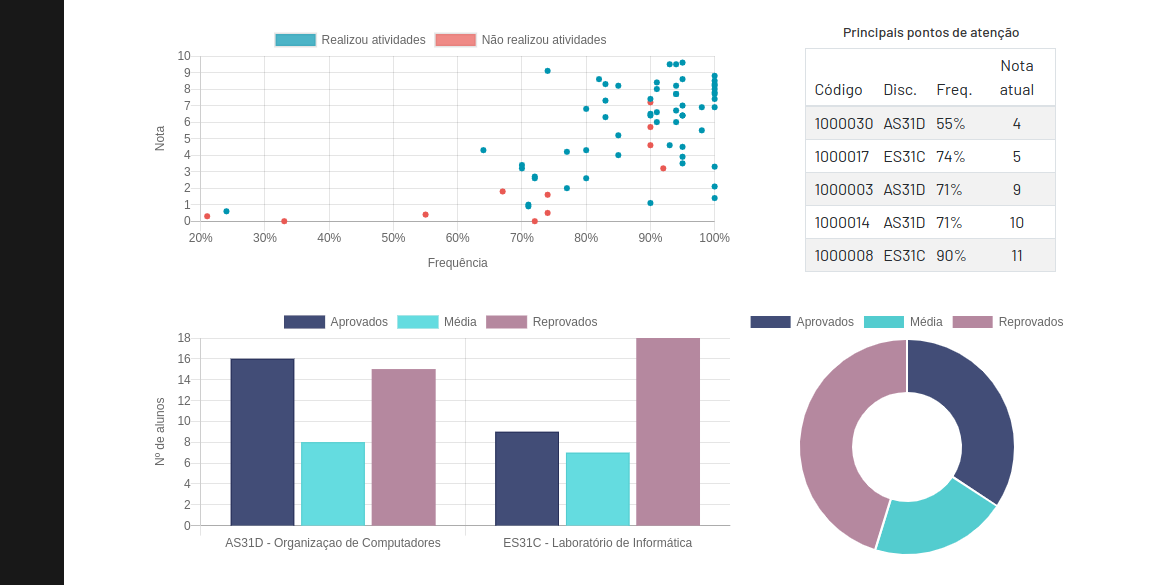
\includegraphics[width=1\textwidth]{./dados/figuras/sistema/sistema-dashboard-2}
    \fonte{Autoria Própria}
    \label{fig:dashboard-2}
\end{figure}

\subsection{Configurações}
\label{ssec:configuracoes}

Seguindo um fluxo da jornada do usuário ao utilizar a ferramenta, após a tela inicial, a próxima a ser acessada em um primeiro acesso ao sistema será a tela de configurações, esta é apresentada na figura  \ref{fig:sistema-configuracoes-1}. 

\begin{figure}[!htb]
    \centering
    \caption{Página de configurações}
    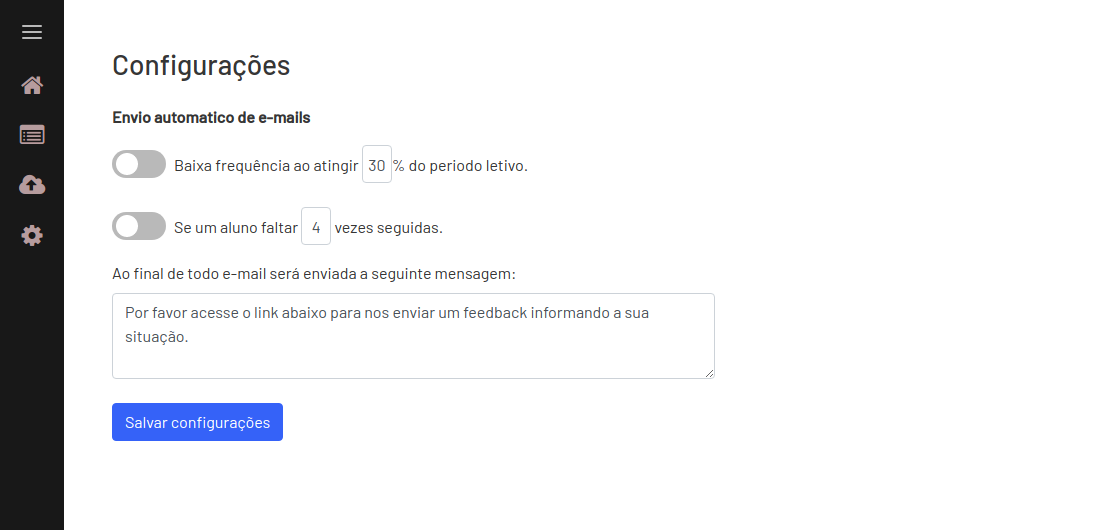
\includegraphics[width=1\textwidth]{./dados/figuras/sistema/sistema-configuracoes-1}
    \fonte{Autoria Própria}
    \label{fig:sistema-configuracoes-1}
\end{figure}

Nesta o usuário pode selecionar dois mecanismos de detecção automática no carregamento de planilhas. 
O primeiro permite que o sistema detecte ao passar uma parte do período letivo os alunos com frequência abaixo do limite de 75\%.
O segundo mecanismo permite a detecção dos alunos que faltaram múltiplas vezes em sequência, o que pode refletir em alguma situação incomum por conta do aluno, como o momento de desistência da disciplina, impedimento médico ou algum outro evento que o impossibilite de participar das aulas.

Com a detecção destes eventos o sistema permite o envio de um e-mail para todos os alunos que se enquadram nessas situações. Desta forma há um campo nesta página para que o usuário possa personalizar a mensagem a ser enviada aos alunos nestes e-mails.
O campo altera a mensagem enviada ao final de todo e-mail, ou seja, a mensagem localizada após todo o texto enviado no e-mail.

Caso habilitados, os mecanismos também dispõe um campo cada, que permite que a mensagem enviada por conta da detecção específica seja personalizada.
Como exemplificado na figura \ref{fig:sistema-configuracoes-2}, as mensagens padrões para os mecanismos são: 

\begin{itemize}
    \item Baixa frequência ao atingir \textit{30\%} do período letivo: O período letivo alcançou \#percentage do semestre e o sistema de prevenção à retenção identificou que sua frequência está abaixo do limite parcial da disciplina.
    \item Se um aluno faltar \textit{4} vezes seguidas: O sistema de prevenção à retenção identificou que você faltou \#times vezes seguidas.
\end{itemize}

\begin{figure}[!htb]
    \centering
    \caption{Página de configurações com campos expandidos}
    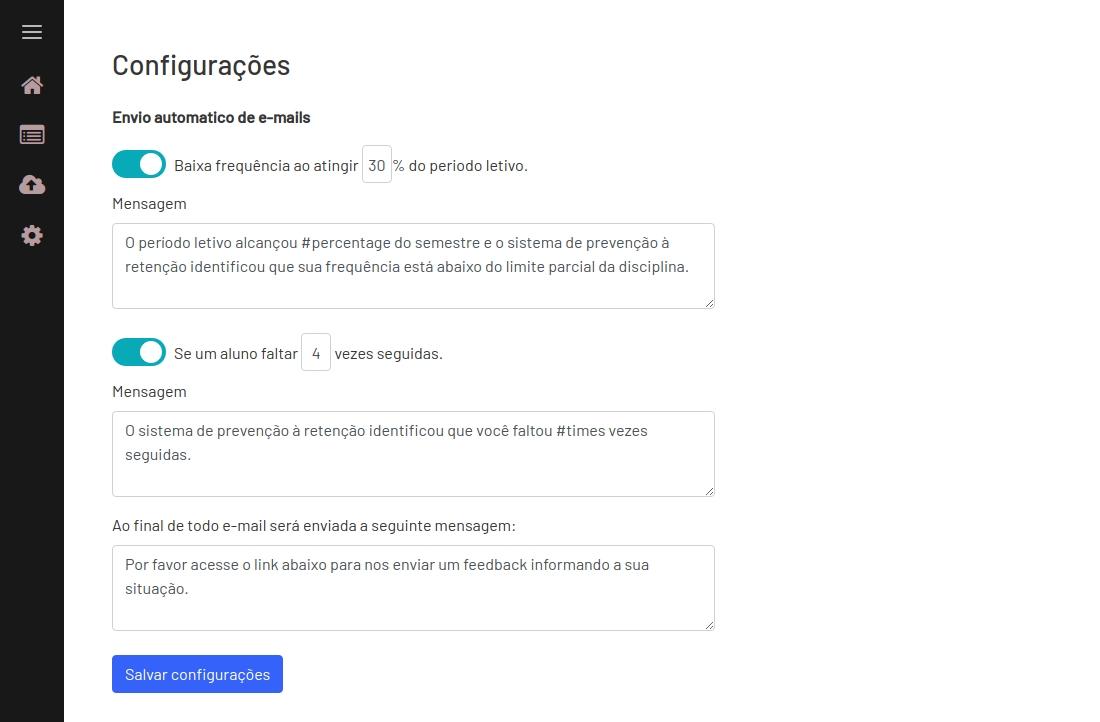
\includegraphics[width=1\textwidth]{./dados/figuras/sistema/sistema-configuracoes-2}
    \fonte{Autoria Própria}
    \label{fig:sistema-configuracoes-2}
\end{figure}

Os termos precedidos pelo símbolo \# representam variáveis que são alteradas automaticamente no envio do e-mail pelo valor gatilho selecionado para o evento. Ou seja, para este caso a expressão \#percentage será substituída por \textit{30\%} e a expressão \#times será substituído por \textit{4}.

\subsection{Upload de Dados}
\label{ssec:uploadDados}

A próxima página do fluxo de uso da ferramenta é a de upload de dados, esta é apresentada na figura \ref{fig:sistema-upload-1}. Nesta tela o usuário pode selecionar a disciplina associada aos dados que serão carregados. 

A \textit{API} em Node.js está preparada para a inserção de novas disciplinas e possui uma rota implementada para esse procedimento, porém o sistema ainda não possui uma tela de cadastro de disciplinas. 
Desta forma algumas disciplinas foram cadastradas a fim de exemplificação. 
Um dos campos esperados na inserção de uma nova disciplina no banco de dados é a data de término do período letivo, utilizado para o cálculo da frequência com base no número de aulas já dadas e faltantes.

Em seguida o usuário deve selecionar o tipo de planilha que será carregada, podendo esta ser de notas e faltas, consolidadas em um arquivo único, ou dados do URI Online Judge Academic.

Caso selecionado a opção \textit{Notas e Faltas} são exibidos campos de pesos, onde o docente deve inserir o peso das avaliações e o peso dos trabalhos para a complementação da nota final dos alunos. 
Os valores são em porcentagem, desta forma a soma dos dois pesos deve equivalente a 100. 
Ao modificar um dos campos de peso automaticamente o peso presente no outro campo será ajustado, complementando-o a 100.

Por fim seleciona-se a planilha a ser submetida e finaliza-se o envio.

\begin{figure}[!htb]
    \centering
    \caption{Página de upload de planilhas}
    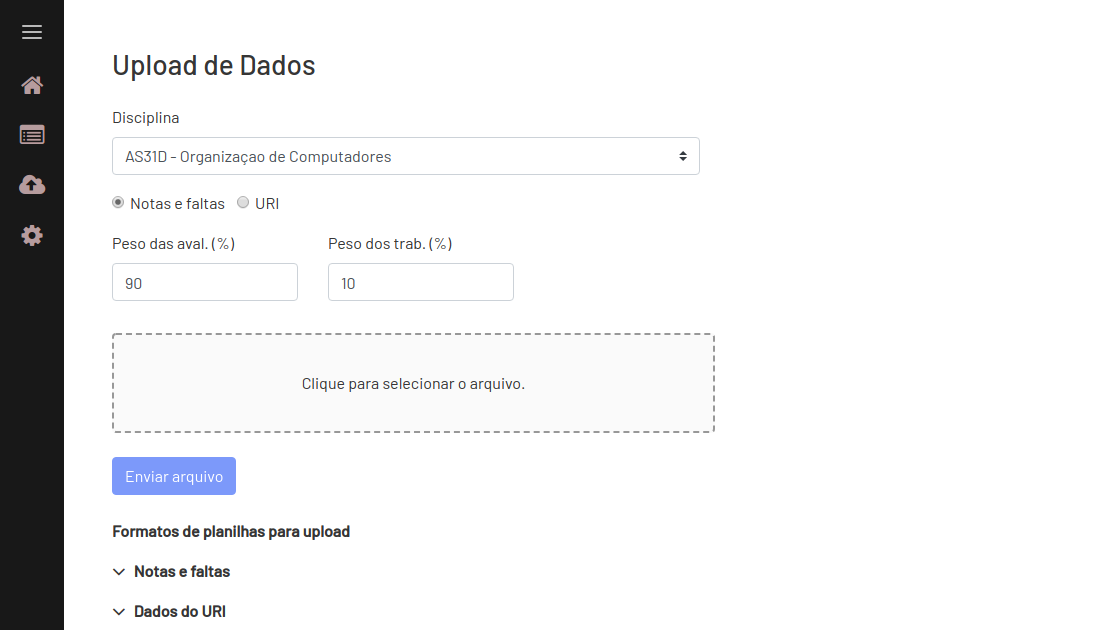
\includegraphics[width=1\textwidth]{./dados/figuras/sistema/sistema-upload-1}
    \fonte{Autoria Própria}
    \label{fig:sistema-upload-1}
\end{figure}

Na parte inferior da página é disposta uma seção guia para os usuários, com os formatos recomendados para as planilhas a serem enviadas. Ao clicar nas setas ao lado de cada opção as opções são expandidas e os \textit{layouts} são apresentados.
A figura \ref{fig:sistema-upload-2} mostra o resultado exibido na tela quando as opções estão expandidas.

\begin{figure}[!htb]
    \centering
    \caption{Página de upload de planilhas com formatos para upload expandidos}
    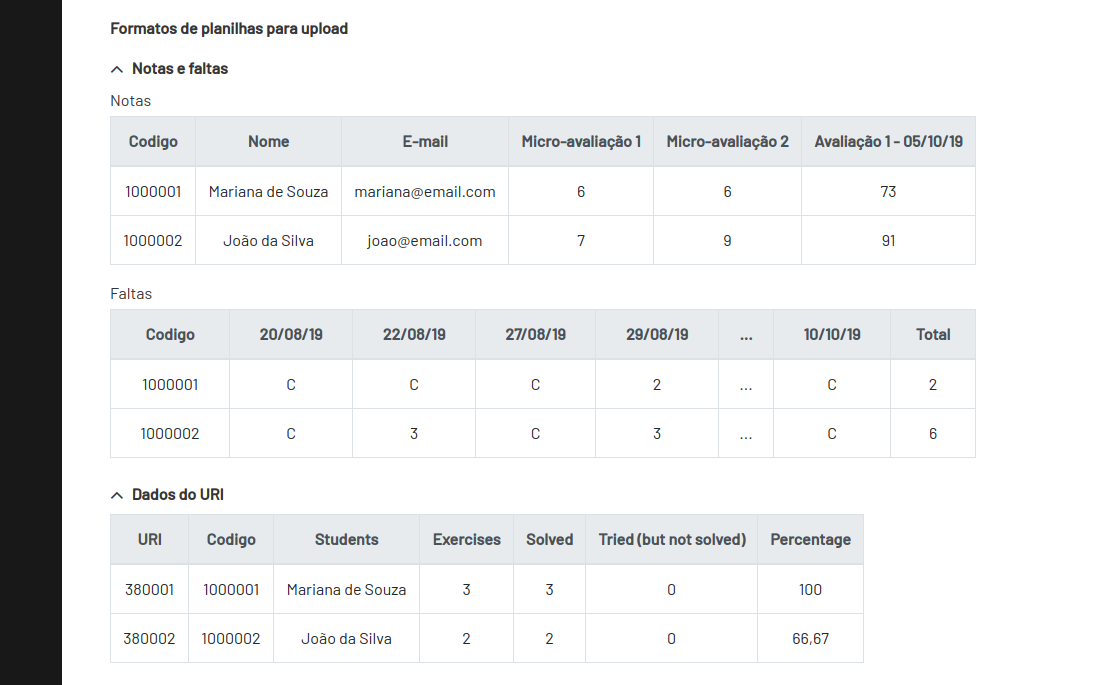
\includegraphics[width=0.8\textwidth]{./dados/figuras/sistema/sistema-upload-2}
    \fonte{Autoria Própria}
    \label{fig:sistema-upload-2}
\end{figure}

Ao finalizar o envio da planilha, internamente o sistema realizará a detecção dos alunos cujos dados se coincidem com os mecanismos assinalados na tela de configurações e exibirá uma página \textit{modal} de alerta com um resumo da situação, solicitando ao usuário a confirmação para o envio dos e-mails a todos os alunos dentro dos perfis detectados.
Caso confirmado, o e-mail é envio pelo endereço de e-mail remetente 
\textit{predicao.academica@gmail.com}, criado somente para a validação deste trabalho, e a mensagem enviada por e-mail aos alunos é construída com base nas mensagens especificadas na tela de configurações anteriormente.
A figura \ref{fig:sistema-upload-3} ilustra a situação de detecção descrita.

\begin{figure}[!htb]
    \centering
    \caption{Detecção de alunos por meio dos mecanismos de comunicação}
    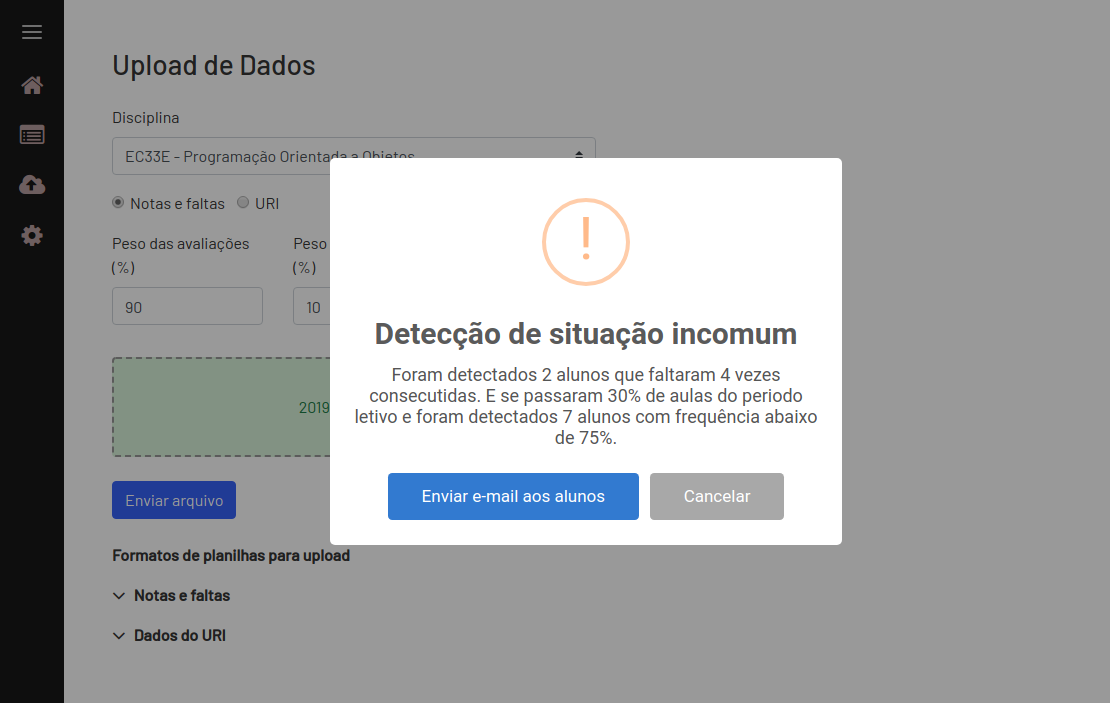
\includegraphics[width=1\textwidth]{./dados/figuras/sistema/sistema-upload-3}
    \fonte{Autoria Própria}
    \label{fig:sistema-upload-3}
\end{figure}

Para fins de validação todos os e-mails atualmente enviados pelo sistema são direcionados para \textit{lucas.franco@alunos.utfpr.edu.br}, mas a plataforma já está preparada para enviá-los para os endereços de e-mail reais dos alunos, quando estes são carregados nas planilha de notas e faltas.

\begin{figure}[!htb]
    \centering
    \caption{Exemplo de e-mail enviado à um aluno pelo sistema de predição automaticamente}
    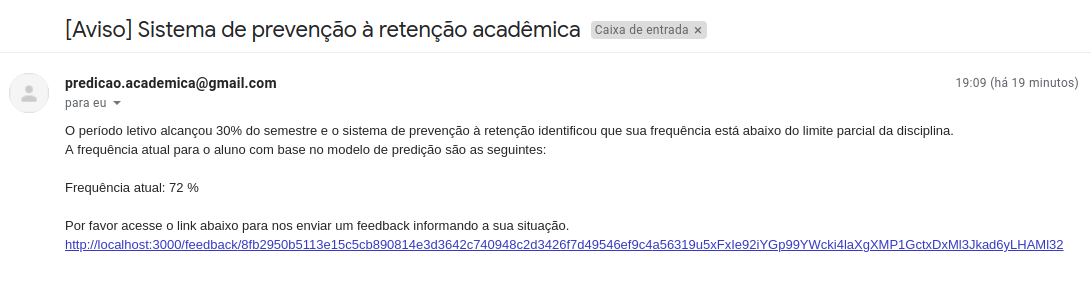
\includegraphics[width=1\textwidth]{./dados/figuras/sistema/sistema-email}
    \fonte{Autoria Própria}
    \label{fig:sistema-email}
\end{figure}

A figura \ref{fig:sistema-email} exibe um exemplo dos e-mails enviados pelo sistema automaticamente por meio da detecção.
Pode-se observar que é enviado junto à mensagem um link para que o aluno acesse. Este link é referente a próxima página a ser descrita, a página de \textit{feedback}.

\subsection{Feedback}
\label{ssec:feedback}

A página de \textit{feedback} é bastante simples e consiste de uma tela que só pode ser acessada pelo link enviado por e-mail.
Ela contém um paragrafo que explica o motivo pelo qual o e-mail lhe foi enviado e o aluno precisa enviar a justificativa, esse também é construído com base nas mensagens definidas na tela de configurações.
Além disso a tela possui um campo para que o aluno envie a justificativa. 
A figura \ref{fig:sistema-feedback} apresenta esta tela.

\begin{figure}[!htb]
    \centering
    \caption{Página de envio de feedback}
    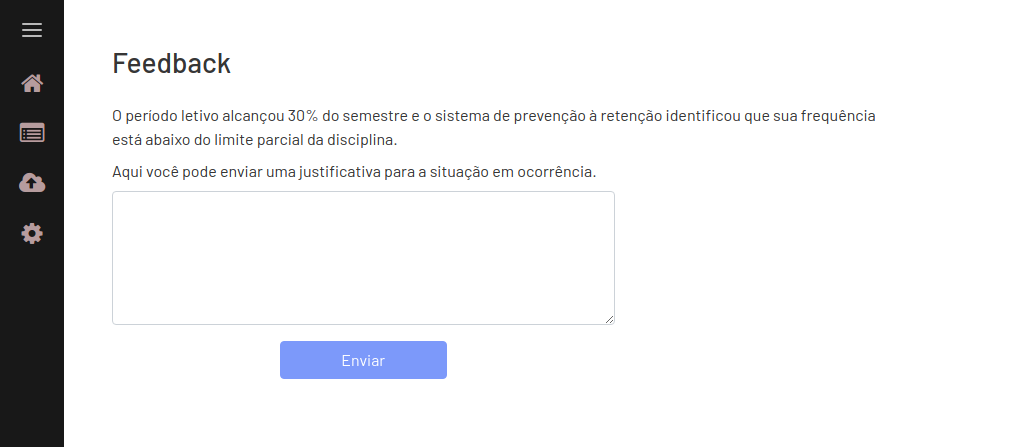
\includegraphics[width=1\textwidth]{./dados/figuras/sistema/sistema-feedback-1}
    \fonte{Autoria Própria}
    \label{fig:sistema-feedback}
\end{figure}

Na \textit{URL} gerada para o acesso a tela de \textit{feedback} são encriptados com a biblioteca \textit{SimpleCrypto} alguns dados que possibilitam identificar e armazenar o texto enviado pelo aluno. 
Entre os dados estão o código identificador do aluno, o código da disciplina e um identificador para o e-mail referente a esta justificativa, gerado ao enviar o e-mail ao aluno.

Não foi-se implementada uma tela de login nesta versão do sistema, mas ao enviar esses dados encriptados na \textit{URL} elimina-se a necessidade de um controle de acesso para os alunos, pois caso não estejam autenticados no sistema estes só poderão acessar as páginas permitidas, que neste caso é somente a tela para o envio do seu \textit{feedback}.

Ao enviar a mensagem o campo para envio da justificativa é desabilitado, assim se o estudante acessar novamente o mesmo link este não conseguirá enviar outra mensagem ou modificar a mensagem enviada.

Uma vez que o aluno envia seu \textit{feedback}, o docente poderá monitorar os e-mails enviados e as respostas recebidas na tela de detalhes do estudante.

O principal meio de acesso a tela de detalhes do estudante é por meio da página de lista. Esta é apresentada a seguir.

\subsection{Lista}

Esta página é responsável pela listagem geral dos dados dos alunos de cada turma. 
Ela é composta por uma caixa de seleção no qual o usuário escolhe a disciplina a ser listada.
A figura \ref{fig:sistema-lista-1} mostra a página de listagem para a disciplina AS31D - Organização de Computadores.

\begin{figure}[!htb]
    \centering
    \caption{Página de listagem de dados}
    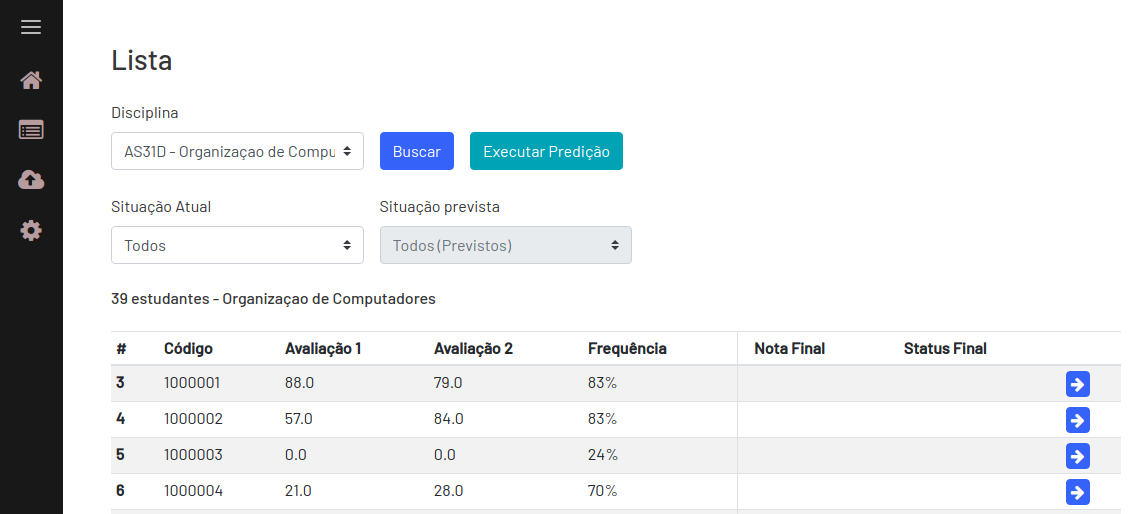
\includegraphics[width=1\textwidth]{./dados/figuras/sistema/sistema-lista-1}
    \fonte{Autoria Própria}
    \label{fig:sistema-lista-1}
\end{figure}

Em seguida estão dispostos dois botões, o primeiro é responsável por solicitar os dados armazenados no banco de dados ao \textit{back-end} em Node.js, e o segundo é responsável por realizar a chamada ao \textit{back-end} em Python, solicitando a execução dos algoritmos de \textit{machine learning} e o retorno das predições. As predições apresentadas no sistema são prevenientes do modelo criado com o algoritmo \textit{Gradient Boosting}.

A sequência de interações realizadas ao pressionar ambos os botões é ilustrada na figura \ref{fig:diagrama-2}.

Logo abaixo da caixa de seleção e botões há dois filtros, um deles é habilitado ao pressionar o botão \textit{Buscar} e permite filtrar pelas regras definidas na subseção \ref{ssec:dashboard}, e são estes: Aprovados, Média (ou limiar) e Reprovados. 
Este filtro considera a nota atual do aluno, calculado com base nas notas das avaliações e atividades.
O segundo filtro é habilitado ao pressionar o botão \textit{Executar Predição}, e permite filtrar seguindo as mesmas regras citadas anteriormente, mas considerando a nota final prevista retornada pelo modelo para os alunos.

Após a execução das predições os campos Nota Final e Status Final são preenchidos com os dados estimados pelos modelos. A figura \ref{fig:sistema-lista-2} apresenta a tela após a execução das predições.
Os alunos que obtiveram uma nota estimada acima de setenta são listados com perfil \textit{Aprovado} e os campos preenchidos são coloridos de verde. 
Para alunos que obtêm notas entre cinquenta e setenta o status apresentado é o \textit{Limiar} e os campos são coloridos de amarelo. 
Por fim os alunos com notas inferiores a 50 são sinalizados com status \textit{Reprovado} e os campos são coloridos com vermelho.

Por mais que o status \textit{Limiar} não traduza diretamente o status final do aluno, o uso desta faixa com 20\% dos pontos (entre 50 e 70) permite à ferramenta uma margem maior entre os status \textit{Aprovado} e \textit{Reprovado}, possibilitando que a determinação delicada do status do aluno com nota prevista na margem seja feita de forma mais branda. 
Porém isso requisita uma análise mais detalhada por conta do docente sobre os alunos que são designados neste perfil.

\begin{figure}[!htb]
    \centering
    \caption{Página de listagem de dados com as predições efetuadas}
    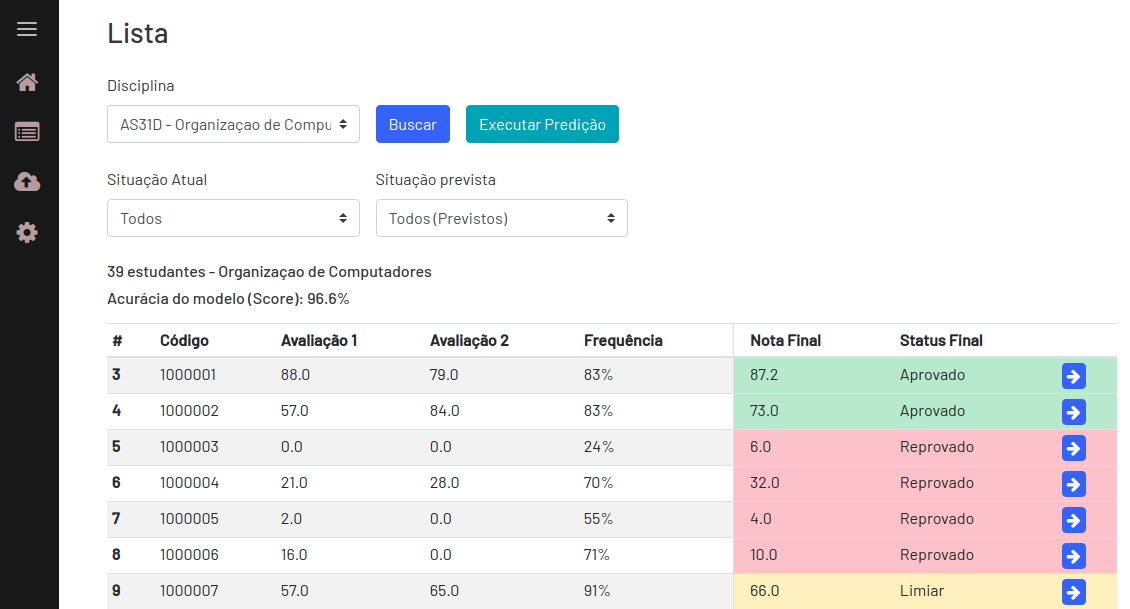
\includegraphics[width=1\textwidth]{./dados/figuras/sistema/sistema-lista-2}
    \fonte{Autoria Própria}
    \label{fig:sistema-lista-2}
\end{figure}

Ainda na tela de listagem, abaixo dos filtros é exibido o número de estudantes listados para a disciplina selecionada e a acurácia/\textit{score} do modelo utilizado para predizer as notas dos alunos.
Ao clicar em um dos botões exibidos na extrema direita de cada linha da tabela é possível acessar a tela de detalhes para o estudante selecionado.

\subsection{Detalhes do Estudante}

A página de detalhes do estudante é responsável por apresentar os dados individuais do aluno selecionado.

Como pode-se visualizar na figura \ref{fig:sistema-detalhes-1}, que ilustra a página de detalhes, esta possui um \textit{card} na parte superior da tela que apresenta o nome e R.A. do aluno, bem como a lista de disciplinas matriculadas com dados inseridos na ferramenta. 
Para cada disciplina são exibidas as notas obtidas pelo aluno até o momento, a sua frequência e a nota final prevista pelo modelo de \textit{machine learning}.

Caso a nota prevista seja igual ou superior a 70 o campo é apresentado em verde e um ícone de \textit{ok} é mostrado, caso a nota esteja entre 50 e 70 o campo é colorido de amarelo com um ícone de atenção.
E para notas inferiores a 50 o campo é apresentado em vermelho com um ícone em forma de \textit{X}.
Semelhante aos indicadores do dashboard apresentados na figura \ref{fig:dashboard-1}.

\begin{figure}[!htb]
    \centering
    \caption{Página de detalhes do estudante}
    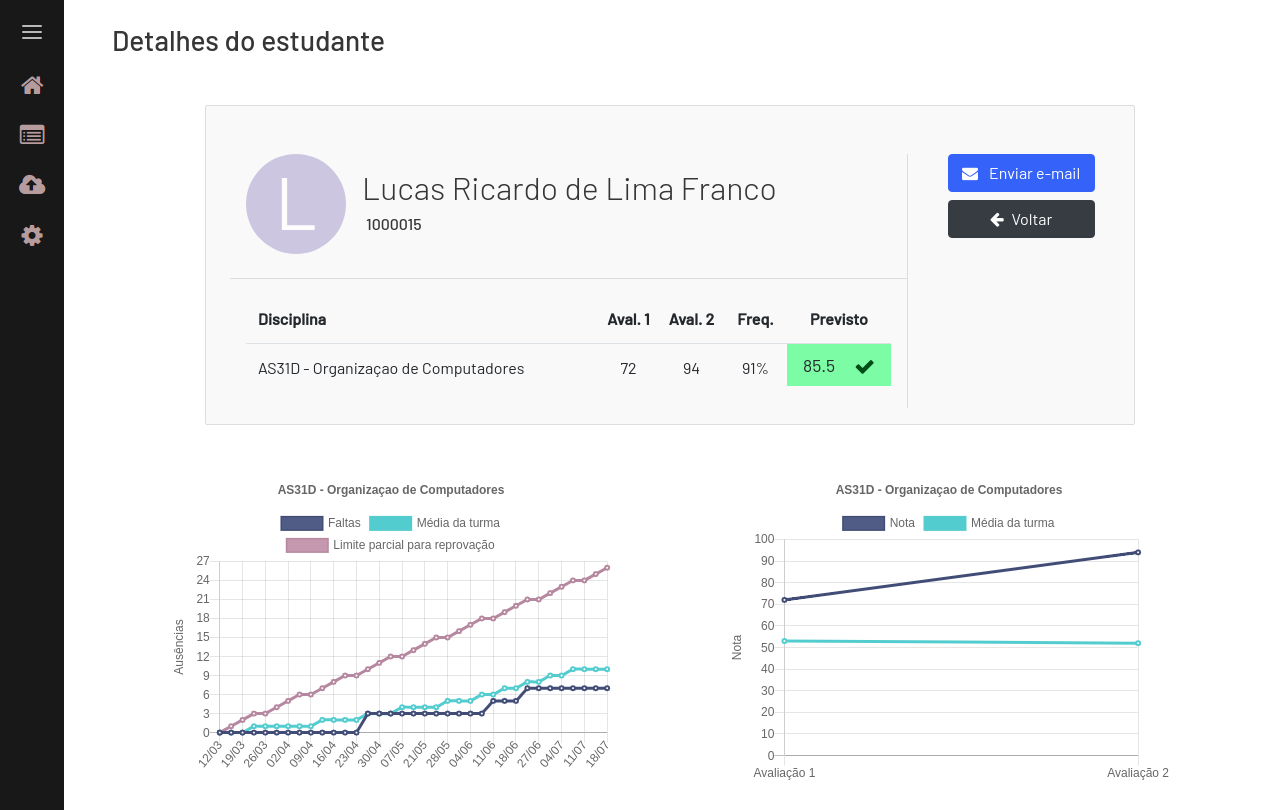
\includegraphics[width=1\textwidth]{./dados/figuras/sistema/sistema-detalhes-1}
    \fonte{Autoria Própria}
    \label{fig:sistema-detalhes-1}
\end{figure}

Abaixo do \textit{card} são gerados dinamicamente gráficos comparativos entre o desempenho do aluno e a média da turma. 
Para cada disciplina vinculada ao aluno é plotado um novo par de gráficos.
Para cada par de gráficos, o primeiro compara o número de ausências do aluno com a média da turma, trazendo também o limite de ausências que um aluno pode ter sem que ocorra a reprovação por faltas.
Já o segundo gráfico ilustra o comportamento das notas do aluno, possibilitando ver se estas estão em crescimento ou declínio, comparando-as com a média de notas da turma.

Retornando ao \textit{card} na parte superior da tela é possível verificar dois botões na sua direita. 
Um deles é utilizado para voltar a tela anterior caso desejado.
O outro é utilizado para realizar o envio de um e-mail personalizado ao aluno apresentado nesta tela, e ao clicar neste botão será apresentado uma página \textit{modal} com um campo para que o usuário insira uma mensagem a ser enviada no e-mail junto de um link gerado automaticamente para que o aluno envie um \textit{feedback}. 
A figura \ref{fig:sistema-detalhes-2} exemplifica a ação ocorrida ao pressionar o botão \textit{Enviar e-mail}.

\begin{figure}[!htb]
    \centering
    \caption{Mensagem personalizada a ser enviada no e-mail por meio da página de detalhes do estudante}
    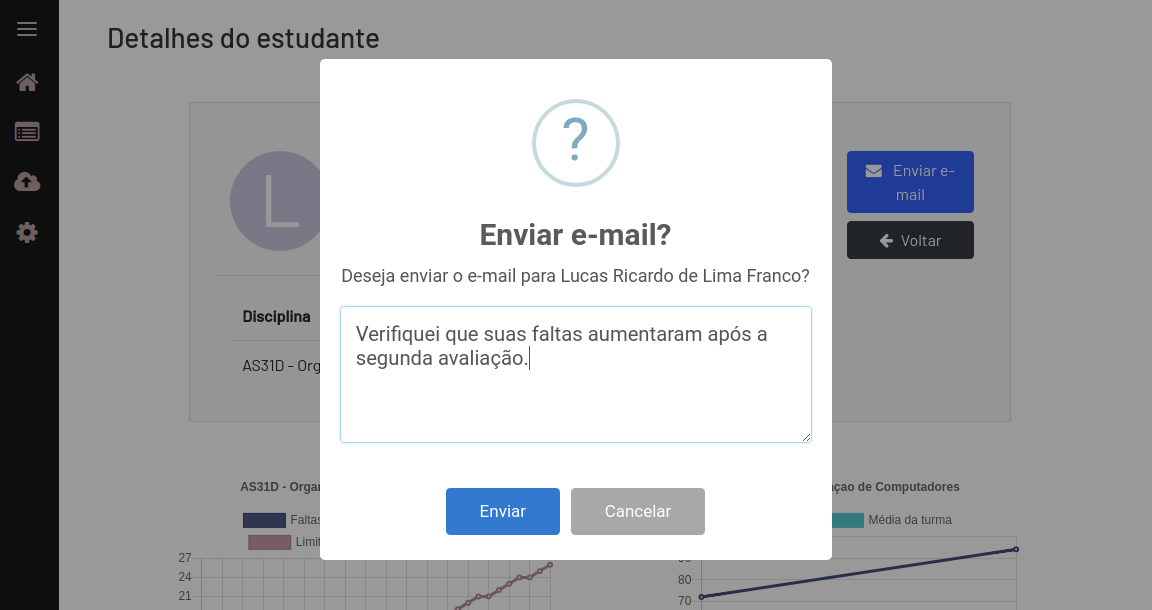
\includegraphics[width=1\textwidth]{./dados/figuras/sistema/sistema-detalhes-2}
    \fonte{Autoria Própria}
    \label{fig:sistema-detalhes-2}
\end{figure}

A figura \ref{fig:sistema-detalhes-3} apresenta o e-mail recebido pelo ação executada anteriormente, nesta é possível verificar que a construção do e-mail se deu com base na mensagem descrita na figura \ref{fig:sistema-detalhes-2}.
Ao final do e-mail se encontra o link para que o aluno acesse e envie o \textit{feedback} solicitado.

\begin{figure}[!htb]
    \centering
    \caption{E-mail enviado por meio da página de detalhes do estudante}
    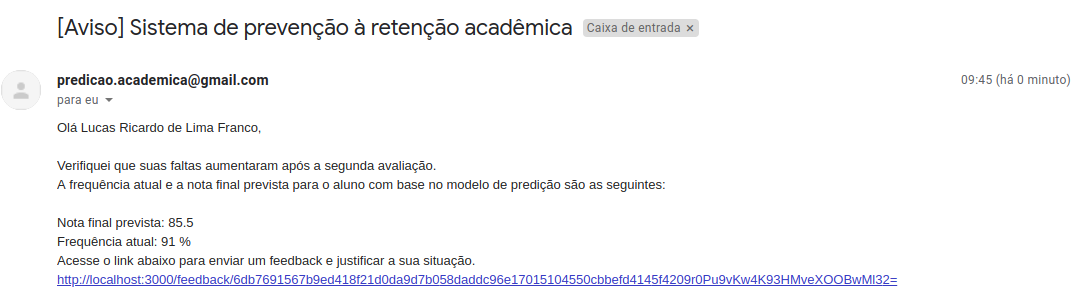
\includegraphics[width=1\textwidth]{./dados/figuras/sistema/sistema-detalhes-3}
    \fonte{Autoria Própria}
    \label{fig:sistema-detalhes-3}
\end{figure}

Por fim a tela de detalhes do estudante permite visualizar a lista de e-mails enviados ao aluno, o status destes, ou seja, se o aluno já o retornou com o seu \textit{feedback} ou se está pendente de resposta. 
Caso o aluno já o tenha respondido é possível ler a justificativa enviada.
Também são exibidas a data e hora de envio dos e-mails e da resposta do aluno, caso existente.

A figura \ref{fig:sistema-detalhes-4} exemplifica a lista de \textit{feedbacks} apresentando uma lista com dois envios de e-mail. 
Esta é ordenada por data de envio, iniciando pelos mais recentes.

O primeiro da lista é referente ao envio do e-mail da figura \ref{fig:sistema-detalhes-3}, que ainda não recebeu uma resposta do aluno.

Já o segundo é referente a uma notificação enviada ao aluno na detecção automática realizada no momento do upload das planilhas, por meio dos mecanismos estabelecidos anteriormente na tela de configurações.
Este recebeu um retorno e pode ser visto no campo \textit{Feedback} da lista.

\begin{figure}[!htb]
    \centering
    \caption{Lista de feedbacks disponível na página de detalhes do estudante}
    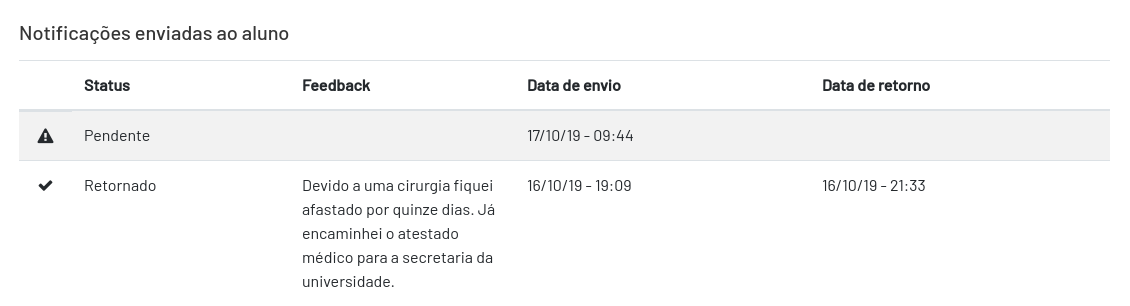
\includegraphics[width=1\textwidth]{./dados/figuras/sistema/sistema-detalhes-4}
    \fonte{Autoria Própria}
    \label{fig:sistema-detalhes-4}
\end{figure}         
\chapter{ANÁLISE DOS RESULTADOS}

\section{MODELOS}

\subsection{Acurácia}

Foram criados dois modelos com cada algoritmo de \textit{machine learning} testado, o primeiro considerando somente uma avaliação e o segundo com notas de duas avaliações.
Os algoritmos utilizados foram o \textit{Gradient Boosting}, \textit{Random Forest} e de Regressão Linear, já descritos anteriormente, e ao realizar o treinamento dos modelos criados com o conjunto de dados disponível foram obtidos seus \textit{scores}, ou acurácias, com o auxilio da biblioteca \textit{Scikit-learn}.

O cálculo do \textit{score} dos modelos foi realizado utilizando o coeficiente de determinação \textit{R\textsuperscript{2}}.
O coeficiente de determinação \textit{R\textsuperscript{2}} é a proporção de variância dos dados que pode ser explicada pelo modelo de regressão. Ela é utilizada para medir o sucesso da predição de uma variável com base em outras variáveis independentes e quanto mais próximo de 1 maior a acurácia do modelo \cite{NAGEKERKE1991}.

A função padrão de \textit{score} do \textit{Scikit-learn} retorna valores entre 0 e 1 para modelos onde a capacidade preditiva é melhor do que a média aritmética dos valores da amostra, ou seja, caso o modelo possua um \textit{score} inferior à 0 o cálculo simples da média dos valores da amostra seria mais preciso que o modelo treinado.

Os \textit{scores} obtidos para os modelos construídos são apresentados na tabela \ref{tab:score-1}, no qual o conjunto 1 representa o conjunto de dados que considera somente uma avaliação e o conjunto 2 leva em conta as duas avaliações.

\begin{table}[!htb]
    \centering
    \caption{Score dos modelos construídos considerando os conjuntos com uma avaliação e duas avaliações}
    \begin{tabular}{ccc}
        \textbf{} & \multicolumn{2}{c}{\textbf{Score}} \\ \hline
        \textbf{Algoritmo} & \textbf{Conjunto 1} & \textbf{Conjunto 2} \\
        Regressão Linear & 99,9\% & 99,7\% \\
        Gradient Boosting & 89,8\% & 97,4\% \\
        Random Forest & 89,4\% & 96,2\% \\ \hline
    \end{tabular}
    \label{tab:score-1}
\end{table}

Percebe-se que os modelos construídos com o algoritmo de regressão linear possuem acurácia muito elevada quando comparado aos outros algoritmos, principalmente para o conjunto 1. 
As tabelas \ref{tab:teste-1} e \ref{tab:teste-2} apresentam os resultados retornados para o conjunto de 20\% de testes para os modelos treinados. 

\begin{table}[!htb]
    \centering
    \caption{Predições realizadas sobre o subconjunto de testes para o conjunto de uma avaliação}
    \begin{tabular}{cccccccc}
        \hline
        \textbf{Algoritmo} & \textbf{1º} & \textbf{2º} & \textbf{3º} & \textbf{4º} & \textbf{5º} & \textbf{6º} & \textbf{7º} \\ \hline
        Gradient Boosting & 64,4 & 9,9 & 64,6 & 44,6 & 17,7 & 2,6 & 14,0 \\
        Random Forest & 65,5 & 10,3 & 67,4 & 42 & 17,6 & 6,6 & 14,6 \\
        Regressão Linear & 68,6 & 10,6 & 56,7 & 31,9 & 25,6 & -0,1 & 20,9 \\
        Valor real & 69,0 & 11,0 & 57,0 & 32 & 26,0 & 0,0 & 21,0 \\ \hline
    \end{tabular}
    \label{tab:teste-1}
\end{table}

\begin{table}[!htb]
    \centering
    \caption{Predições realizadas sobre o subconjunto de testes para o conjunto de duas avaliações}
    \begin{tabular}{ccccccccllllll}
        \hline
        \textbf{Algoritmo} & \textbf{1º} & \textbf{2º} & \textbf{3º} & \textbf{4º} & \textbf{5º} & \textbf{6º} & \textbf{7º} & \textbf{8º} & \textbf{9º} & \textbf{10º} & \textbf{11º} \\ \hline
        Gradient Boosting & 75,4 & 63,6 & 29,4 & 26,4 & 66,9 & 82,2 & 25,5 & 0,0 & 0,0 & 78,3 & 71,5 \\
        Random Forest & 81,3 & 60,5 & 27,1 & 25,7 & 63,4 & 76,2 & 26,2 & 0,6 & 0,1 & 78,8 & 71,4 \\
        Regressão Linear & 79,5 & 59,1 & 22,8 & 18,1 & 65,3 & 76,9 & 27,7 & -0,1 & 0,5 & 79,7 & 68,7 \\
        Valor real & 80,0 & 60,0 & 25,0 & 18,0 & 64,0 & 77,0 & 29,0 & 0,0 & 0,0 & 80,0 & 69,0 \\ \hline
    \end{tabular}
    \label{tab:teste-2}
\end{table}

Dentre os algoritmos, o \textit{Gradient Boosting} e \textit{Random Forest} são considerados mais adequados para um volume pequeno de dados de treinamento e mais robustos quanto a \textit{overfitting} quando comparados aos algoritmos de regressão linear.
Desta forma, a fim de verificar a acurácia dos modelos para diferentes situações foi-se executada a validação cruzada dos modelos, que divide o conjunto de dados em subconjuntos, treina e testa o modelo, retornando a acurácia média e desvio padrão dos diferentes subconjuntos.

A tabela \ref{tab:validacao-cruzada} apresenta a média das acurácias dos modelos e o desvio padrão entre as acurácias obtidas com o \textit{Scikit-learn}, considerando uma validação cruzada de três subconjuntos.

\begin{table}[!htb]
    \centering
    \caption{Scores médios e desvios padrões obtidos com a validação cruzada em três subconjuntos}
    \begin{tabular}{ccccc}
      \textbf{} & \multicolumn{2}{c}{\textbf{Conjunto 1}} &   \multicolumn{2}{c}{\textbf{Conjunto 2}} \\ \hline
        \textbf{Algoritmo} & \textbf{Score} & \textbf{D. Padrão} & \textbf{Score} & \textbf{D. Padrão} \\ \hline
        Gradient Boosting  & 95,8\% & $\pm 3,5$\% & 92,1\% & $\pm 0,9$\% \\
        Random Forest & 90,0\% & $\pm 5,6$\% & 88,6\% & $\pm 2,3$\% \\
        Regressão Linear & 85,8\% & $\pm 9,7$\% & 75,1\% & $\pm 0,7$\%  \\ \hline
    \end{tabular}
    \label{tab:validacao-cruzada}
\end{table}

Com a validação cruzada foi possível observar um melhor desempenho do algoritmo \textit{Gradient Boosting} para ambos os casos, retornando também um menor desvio padrão para o conjunto 1.
Dentre os três algoritmos, o \textit{Random Forest} obteve acurácias intermediárias e a regressão linear foi a que retornou o pior desempenho.

Devido ao algoritmo \textit{Gradient Boosting} apresentar os melhores resultados na maioria dos casos, este foi empregado como a técnica utilizada para retornar as predições em toda a plataforma desenvolvida neste trabalho.

\subsection{Importância}

As tabelas \ref{tab:importanciaGradient} e \ref{tab:importanciaRandom} mostram a importância das variáveis para os algoritmos \textit{Gradient Boosting} e \textit{Random Forest} para o conjunto de duas avaliações.
Nelas é possível observar que para o conjunto de dados utilizados a nota da segunda avaliação tem uma influência muito grande no resultado final das predições, possuindo importâncias de 79,9\% e 55,7\% para os dois modelos, respectivamente.

Os modelos divergem quanto a segunda variável com maior influência sobre a predição, mostrando que tanto a nota do primeiro trabalho quanto a nota da primeira avaliação podem ser importantes nesse contexto.

A frequência do aluno ficou em 4º lugar com 3,2\% na lista do primeiro algoritmo e em 3º lugar com 14,5\% para o segundo, apresentando certa diferença no nível de importância mas mostrando que em ambos os casos esta variável ainda se faz presente nas predições.

Em ambos os modelos as variáveis com menor importância foram as notas do segundo e terceiro trabalhos, com influências de 1,7\% ou menos nas estimativas.

Já a tabela \ref{tab:importanciaUmaProva} lista as variáveis e suas importâncias considerando alunos que só realizaram uma avaliação. Neste caso o nível de incerteza dependerá do padrão da disciplina. Caso o previsto seja a aplicação de três avaliações, o nível de incerteza se torna maior quanto à nota final dos alunos, pois há mais variáveis desconhecidas do que conhecidas para se realizar a predição, por exemplo, conhece-se a nota da primeira avaliação mas não da segunda e terceira avaliações.
Neste caso, pode-se verificar que a nota da primeira avaliação está diretamente relacionada a nota final prevista para o aluno, com 89,6\% e 92,7\% de importância, respectivamente, para as predições realizadas pelo \textit{Gradient Boosting} e pelo \textit{Random Forest}.

Ao comparar as tabelas \ref{tab:importanciaGradient} e \ref{tab:importanciaRandom} com a tabela \ref{tab:importanciaUmaProva} é possível observar que para o conjunto de dados que possui notas de duas avaliações a importância se diluiu mais entre as \textit{features} disponíveis, enquanto que para dados com somente uma avaliação a importância se concentrou na nota da avaliação realizada. 
Complementar a isto, os dados dos exercícios da plataforma URI tiveram uma participação muita baixa nas estimativas dos modelos, com cerca de 1,0\% de influência para ambos os algoritmos.

Em seguida tem-se a tabela \ref{tab:importanciaComDatas}, que mostra o resultado de um teste realizado considerando como \textit{features} cada um dos dias de aula.
Foi possível observar que individualmente as aulas não tiveram participação considerável na predição das notas finais dos alunos, com um máximo de 0,2\% por aula individual e total de 0,9\% ao somar as importâncias de todas as aulas do modelo construído com o \textit{Gradient Boosting}, que foi o modelo que retornou maior influência destas variáveis.

Por fim a tabela \ref{tab:coef-linear} mostra os coeficientes determinados para a equação linear gerada pelo algoritmo de regressão linear. 
E nesta é possível observar uma maior distribuição da influência entre as variáveis, apresentando, como os outros algoritmos, um coeficiente mais elevado para a a nota da segunda avaliação, seguida da nota da primeira avaliação, com 0,473 e 0,407, respectivamente, somando um coeficiente conjunto de 0,88 para as avaliações. 
Já para os trabalhos os coeficientes somados representam um valor de 0,116. 
O restante fica por conta da frequência e da porcentagem de exercícios do URI resolvidos. 
Este último obteve um coeficiente negativo, porém muito pequeno, o que se torna praticamente irrelevante para a estimativa da nota final.

\section{IMPLEMENTAÇÃO}

Os resultados obtidos acerca da plataforma desenvolvida foram mais subjetivos, mas é possível visualizar os potenciais que a ferramenta têm para o auxílio dos usuários na análise dos dados acadêmicos.

\subsection{Dashboard}

Com o dashboard implementado é possível extrair alguns \textit{insights} sobre os dados. 
O gráfico temporal apresentado na figura \ref{fig:dashboard-1} possibilita verificar a proporção de faltas da turma como um todo, e caso a linha de faltas da turma ultrapasse a linha que representa o limite permitido de faltas, o profissional pode tomar ações para compreender em detalhes quais os motivos que levam a esse acontecimento.
Já com os indicadores da parte superior da mesma página, pode-se ter uma visão geral das turmas cadastradas ou de uma turma específica selecionado-a na caixa de seleção flutuante presente à direita.

A partir do gráfico de dispersão do dashboard, figura \ref{fig:dashboard-2}, pode-se verificar visualmente o nível de correlação presente entre a frequência e as notas dos alunos, e caso a influência dos trabalhos na nota final seja explícita o profissional pode tomar ações ou apresentar este gráfico aos alunos, argumentando e influenciando-os a seguir o perfil que tende a receber melhores notas.

No mesmo gráfico pode-se verificar que há alunos com frequências próximas ou iguais a 100\% mas com notas abaixo da média para aprovação, desta forma é possível acessar estes alunos a fim de averiguar quais os motivos que os levam a não obterem desempenho tão bons na disciplina.
Com isso pode-se descobrir lacunas no método pedagógico utilizado pelo docente e oportunidades de utilização de recursos para a melhoria do aprendizado, como os alunos monitores com um maior foco nestes alunos.

Ainda no dashboard, o gráfico de barras permite uma análise rápida das notas do alunos nas disciplinas e a comparação entre elas, assim pode-se identificar a proporção de alunos com um bom, médio e baixo desempenho, apurando também as disciplinas com menor aproveitamento por conta dos alunos.

\subsection{Predição, Feedback e Mecanismos de Detecção}

A predição das notas dos alunos em conjunto com a detecção de situações incomuns complementam o sistema proposto e desenvolvido neste trabalho, que tem como objetivo fornecer ferramentas para que os profissionais possam analisar dados acadêmicos e tomar algumas ações simples sem a necessidade de muitos esforços manuais.

A página de detalhes do estudante proporciona ao docente uma visão da situação atual do aluno, permitindo nela comparar o aluno à média, tanto em faltas quanto em notas. 
Esta é uma forma de investigar um aluno a fim de identificar padrões no seu comportamento, como a diminuição das notas coincidentemente na época do período letivo que o aluno mais obteve faltas.

Ainda na mesma página o profissional poderá submeter uma notificação ao aluno, solicitando um \textit{feedback}. 
Este recurso foi idealizado para o uso em situações que demandam uma advertência, mas ele não é restrito a isso. 
Caso o docente observe alguma variação no perfil dos alunos, este pode pedir um \textit{feedback} também em uma situação ainda considerada adequada para o aluno.
Um exemplo de padrão que o professor pode identificar é a ausência de determinados alunos no mesmo dia da semana. 
Deduz-se então que algum evento em especial pode estar ocorrendo nestes dias e o docente pode enviar um e-mail aos alunos a fim de comprovar seu \textit{insight}.

Um dos objetivos almejados com a possibilidade de os alunos enviarem \textit{feedbacks} é verificar se a comunicação com os alunos pode ser uma forma de conscientização e consequentemente melhores resultados no desempenho dos alunos.

Observou-se com a base de dados utilizada neste trabalho que existem diferentes perfis de estudantes e este sistema é destinado a atingir a parcela de alunos que possui dedicação aos estudos mas por algum motivo sob o domínio do professor não consegue obter um bom desempenho e devido a isto possui perfil tendencioso a desistência ou reprovação nas disciplinas.

Como descrito anteriormente, o algoritmo selecionado para a predição das notas dos alunos foi o \textit{Gradient Boosting}.
Com ela utilizando uma base histórica tornou-se possível estimar o desempenho dos alunos, a fim de tomar ações e inibir a retenção acadêmica antes do seu acontecimento.

Em contrapartida observou-se que o algoritmo de regressão linear determinou o coeficientes da sua equação linear com valores muito semelhantes aos pesos para avaliações e trabalhos definidos no carregamento dos dados na ferramenta.
Os pesos utilizados no momento do carregamento foram 0,9 para as avaliações e 0,1 para os trabalhos e os coeficientes retornados pelo algoritmo para as avaliações e para os trabalhos foram 0,880 e 0,116, respectivamente, o que comprovou uma boa capacidade de modelar o método de avaliação por conta do algoritmo.
Para dados que não seguiam um comportamento linear o \textit{Gradient Boosting} se mostrou melhor.

O sistema construído segmenta os alunos em três perfis, o primeiro com mais chances de aprovação na disciplina, o segundo com estimativas medianas e o terceiro com maiores riscos de reprovação. 
Com isso o profissional pode selecionar um perfil específico e atuar sobre os alunos contidos nele com o intuito de melhorar suas situações e colaborar com a transição destes para perfis mais positivos.            
% % RESULTADOS-------------------------------------------------------------------

\chapter{CRONOGRAMA}

O cronograma foi construído com base no método CRISP-DM, apresentado na seção \ref{ssec:crisp}, que será utilizado para definir a sequência de tarefas que serão realizadas durante o período de trabalho. 

Devido a natureza iterativa do modelo CRISP-DM, foram acrescentados períodos de trabalho extra para as atividades que requerem revisão e ajustes durante o desenvolvimento do projeto.
Como exemplo de tarefas tem-se a \textit{definição de objetivos de negócio}, que podem sofrer alterações conforme o resultado obtido na tarefa de \textit{análise dos dados}. 
De forma semelhante ocorre a \textit{seleção das técnicas de mineração de dados}, que dependerão da assertividade apresentada pelas técnicas com o conjunto de dados utilizado no trabalho.

O cronograma é apresentado à seguir, na \autoref{tab:cronograma}.

\begin{landscape}
\begin{table}[!htb]
    \centering
    \caption[Cronograma]{Cronograma}
    \tiny
    \label{tab:cronograma}
    \begin{tabular}{*{40}{c}}
        \topline
          \\
              \multicolumn{2}{l}{}
            & \multicolumn{4}{c|}{Novembro}
            & \multicolumn{4}{c|}{Dezembro} 
            & \multicolumn{4}{c|}{Fevereiro} 
            & \multicolumn{4}{c|}{Março} 
            & \multicolumn{4}{c|}{Abril} 
            & \multicolumn{4}{c|}{Maio} \\
            
        \hline
          \multicolumn{2}{l}{}
            & 1 & 2 & 3 & 4 & 
            1 & 2 & 3 & 4 &
            1 & 2 & 3 & 4 &
            1 & 2 & 3 & 4 &
            1 & 2 & 3 & 4 &
            1 & 2 & 3 & 4 &\\
            
        \midrule
            \multirow{2}{*}{\begin{tabular}[c]{@{}l@{}} Levantamento \\ bibliográfico\end{tabular}} 
            & Estudo de Técnicas de MD      & X & X & & & \\\cmidrule(r){2-26}
            & Estudo de Ferramentas         & & X & X & & \\\cmidrule(l){1-26}
            
            \multirow{2}{*}{\begin{tabular}[c]{@{}l@{}} Entendimento \\ do negócio \end{tabular}}
            & Definir objetivos de negócio  & & & X & X & & & & & & X &\\\cmidrule(r){2-26}
            & Definir objetivos de MD       & & & & X & X & & & & & & X &   \\\cmidrule(l){1-26}
         
            \multirow{3}{*}{\begin{tabular}[c]{@{}l@{}} Entendimento \\ dos dados \end{tabular}} 
            & Scripts Coleta de dados  & & & & X & X & \\\cmidrule(r){2-26}
            & Coleta inicial dos dados      & & & & & X & X & &   \\\cmidrule(r){2-26}
            & Análise dos dados             & & & & & & X & X & & & & & & & X & X & \\\cmidrule(l){1-26}
            
            \multirow{3}{*}{\begin{tabular}[c]{@{}l@{}} Preparação \\ dos dados \end{tabular}} 
            & Scripts Prep. dos dados           & & & & & & X & X & X & \\\cmidrule(r){2-26}
            & Seleção dos dados                 & & & & & & & X & & & & & & & & & X & \\\cmidrule(r){2-26}
            & Limpeza e construção              & & & & & & & & X & X & & & & & & & & X &\\\cmidrule(r){2-26}
            & Integração e Formatação           & & & & & & & & & X & X & & & & & & & & X &\\\cmidrule(l){1-26}
            
            \multirow{4}{*}{\begin{tabular}[c]{@{}l@{}} Modelagem \end{tabular}}
            & Seleção de técnicas de MD     & & & & & & & & & X & & & & & & & & X & \\\cmidrule(r){2-26}
            & Construção dos modelos        & & & & & & & & & & X & X & X & & & & & & & X & X & \\\cmidrule(r){2-26}
            & Testes empíricos              & & & & & & & & & & & & X & X & X & & & & & & X & X &\\\cmidrule(l){1-26}

            \multirow{3}{*}{\begin{tabular}[c]{@{}l@{}} Validação \\ dos modelos \end{tabular}}
            & Avaliação dos objetivos       & & & & & & & & & & & & & & & X & X & & & & & X & \\\cmidrule(r){2-26}
            & Avaliação da acurácia         & & & & & & & & & & & & & & & X & X & & & & & X & \\\cmidrule(r){2-26}
            & Revisão dos modelos           & & & & & & & & & & & & & & & & & X \\\cmidrule(l){1-26}
            
            \multirow{2}{*}{\begin{tabular}[c]{@{}l@{}} Implantação \end{tabular}}
            & Sistema web                   & & & & & & & & & & & & & & & X & X & X & X & X & \\\cmidrule(r){2-26}
            & Apresentação dos dados           & & & & & & & & & & & & & & & & X & X & X & X & X & \\\cmidrule(r){2-26}
            & Mecanismos automatizados      & & & & & & & & & & & & & & & & & & & X & X & X & X \\\cmidrule(l){1-26}
         
            \multirow{1}{*}{\begin{tabular}[c]{@{}l@{}} Conclusão \end{tabular}}
            &               & & & & & & & & & & & & & & & & & & & & & & & X & \\
    
        \bottomrule
    \end{tabular}
\end{table}
\end{landscape}


\chapter{CONCLUSÃO}
\label{chap:conclusao}

O desenvolvimento deste trabalho possibilitou compreender o impacto que a retenção acadêmica possui para as universidades brasileiras, e refletir sobre quais são as formas de contribuir para a redução este problema. 
A retenção acadêmica é uma das variáveis relacionadas à evasão acadêmica e uma das formas de se iniciar a trabalhar sobre a evasão é observar anteriormente o fenômeno da retenção acadêmica.

Foi-se então implementado um ``ecossistema'' de análise de dados acadêmicos para o fornecimento de mecanismos que permitam atuar sobre a retenção acadêmica e estimar o status final dos alunos.

A ferramenta desenvolvida neste trabalho possibilita que docentes tenham uma maior aplicação dos dados que possuem, permitindo que estes carreguem dados das disciplinas ministradas e a partir disso utilize mecanismos para comunicar-se com alunos em perfil tendencioso à retenção, a fim de compreender e impedir seu acontecimento.

Com o estudo realizado sobre os dados de alunos da UTFPR - Campus Cornélio Procópio foi possível implementar modelos preditivos que atuam a fim de antecipar a retenção acadêmica ocorrida principalmente devido a ausências e assim garantir que os docentes engajados possam realizar tomadas de decisão para auxiliar os alunos na regularização das suas situações. 

Dentre os algoritmos de mineração de dados empregados o \textit{Gradient Boosting} se mostrou mais adequado para o conjunto de dados utilizado, com uma acurácia obtida entre 89,8\% e 97,4\%.

Como oportunidades de trabalhos futuros tem-se a exploração em mais detalhes de dados dos alunos, dentre esses os dados sociais, como a idade, gênero, histórico familiar e educacional, e os de cunho financeiro como a renda familiar e o recebimento de bolsas de auxílio.
Com estes dados é possível ampliar o objeto de estudo deste trabalho para além da retenção, alcançando também o âmbito da evasão acadêmica, que possui uma natureza muito mais subjetiva.

Outra possibilidade de trabalho é análise de diferentes tipos de cursos, comparando por exemplo cursos presenciais e de educação à distância, no qual a frequência não é um dos fatores chave para a aprovação.

O acesso de assistentes psicopedagógicos na ferramenta também é uma possibilidade de expansão, desta forma profissionais com um \textit{background} mais específico na interação com os alunos poderiam realizar um trabalho mais direcionado aos alunos que foram identificados com risco de retenção.

\postextual
% INSERE ELEMENTOS PÓS-TEXTUAIS
% REFERÊNCIAS------------------------------------------------------------------

% Carrega o arquivo "base-referencias.bib" e extrai automaticamente as referências citadas

\bibliography{./base-referencias}
\bibliographystyle{abntex2-alf} % Define o estilo ABNT para formatar a lista de referências
% OBSERVAÇÕES------------------------------------------------------------------
% Este arquivo não precisa ser alterado.

% % APÊNDICES--------------------------------------------------------------------

\begin{apendicesenv}
\partapendices

% Primeiro apêndice------------------------------------------------------------
\chapter{Nome do apêndice} % Edite para alterar o título deste apêndice
\label{chap:apendiceA}

Lembre-se que a diferença entre apêndice e anexo diz respeito à autoria do texto e/ou material ali colocado.

Caso o material ou texto suplementar ou complementar seja de sua autoria, então ele deverá ser colocado como um apêndice. Porém, caso a autoria seja de terceiros, então o material ou texto deverá ser colocado como anexo.

Caso seja conveniente, podem ser criados outros apêndices para o seu trabalho acadêmico. Basta recortar e colar este trecho neste mesmo documento. Lembre-se de alterar o "label"{} do apêndice.

Não é aconselhável colocar tudo que é complementar em um único apêndice. Organize os apêndices de modo que, em cada um deles, haja um único tipo de conteúdo. Isso facilita a leitura e compreensão para o leitor do trabalho.

% Novo apêndice----------------------------------------------------------------
\chapter{Nome do outro apêndice}
\label{chap:apendiceB}

conteúdo do novo apêndice

\end{apendicesenv}
 
% % ANEXO------------------------------------------------------------------------

\begin{anexosenv}
\partanexos

% Primeiro anexo---------------------------------------------------------------
\chapter{Nome do anexo}     % edite para alterar o título deste anexo
\label{chap:anexoA}

Lembre-se que a diferença entre apêndice e anexo diz respeito à autoria do texto e/ou material ali colocado.

Caso o material ou texto suplementar ou complementar seja de sua autoria, então ele deverá ser colocado como um apêndice. Porém, caso a autoria seja de terceiros, então o material ou texto deverá ser colocado como anexo.

Caso seja conveniente, podem ser criados outros anexos para o seu trabalho acadêmico. Basta recortar e colar este trecho neste mesmo documento. Lembre-se de alterar o "label"{} do anexo.

Organize seus anexos de modo a que, em cada um deles, haja um único tipo de conteúdo. Isso facilita a leitura e compreensão para o leitor do trabalho. É para ele que você escreve.

% Novo anexo-------------------------------------------------------------------
\chapter{Nome do outro anexo}
\label{chap:anexoB}

conteúdo do outro anexo

\end{anexosenv}


\end{document}
